\documentclass[12pt]{extarticle}

\usepackage{hyperref}
\usepackage[]{algorithm2e}
\usepackage{amsfonts}
\usepackage{amsmath, amsthm, amssymb}
\usepackage{graphicx, wrapfig}
\usepackage{float}
\usepackage{caption}
\usepackage{subcaption}
\usepackage{verbatim}

\renewcommand{\refname}{ References}

\oddsidemargin = -10pt
\topmargin = 0pt
\headheight = 0pt
\headsep = 0pt
\textheight = 660pt
\textwidth = 480pt
\marginparsep = 5pt
\marginparwidth = 0pt
\footskip = 70pt
\marginparpush = 5pt 
\paperwidth = 597pt
\paperheight = 845pt


\title {\bf Calculating mutual information in metric spaces \\ BSc Final-year project}
\author{\large Kristian Krastev (kk12742) \\ Supervised by Dr. Conor Houghton}
\date{}

\begin{document}
\maketitle
\newpage
\tableofcontents

\newpage
\addcontentsline{toc}{section}{Abstract}
\section*{Abstract}
\noindent
Mutual information is a quantity that tells us how much knowledge of
one variable reduces uncertainty about another one \cite{Thomas, Shannon}.
It is a useful tool in many applications that rely on
statistical models - for example in various types of clustering where
one aims to maximise dependency within a partition. Typically, as with
most information theory quantities, mutual information is estimated
for variables that are either discrete or take values in a coordinate
space. However, many important data types have distance metrics or
measures of similarity, but no coordinates on them and thus no obvious
integration measure. Datasets of this type are collected from
electrophysiological experiments in neuroscience and gene expression
data in genetics and biochemistry, but also in other fields like image
analysis and data retrieval.\\

\noindent
The purpose of this project is to implement and test an estimator for
calculating mutual information between data, where one or both variables come
from a metric space without coordinates. The model estimator itself has been
described in \cite{Houghton}, but not implemented and tested yet. It aims to
provide a simple approach to the Kozachenko-Leonenko estimator for
mutual information \cite{Kozachenko-Leonenko}, that extends it in order to apply to the broader
class of metric-space data.\\

\noindent
The model is particularly relevant to neuroscience because it addresses the
problem of calculating information theory quantities from the similarity
measures on the space of spike trains. This is the application that motivates it
and will serve as the main source of data, used to test and adjust it.\\

\noindent
Application software will be developed in Python. It is the preferred choice
over MATLAB for example, because it is a modern high-level language with nice
syntax and structure that supports various coding styles. It also has the
analogous libraries and packages relevant to the task - NumPy, SciPy, matplotlib
and so on. In addition to this, it offers interfaces to other tools for computational
neuroscience and mathematics, which can be useful for the project.\\

\noindent
The implementation will first apply the suggested model to fictive
data - both discrete and metric-space. Results will then be analysed
and used to test it on real neuroscientific data. The proposed thesis
will aim to investigate the model's correctness and evaluate its
performance on various types of datasets.\\

\newpage
\section{Background}
\subsection{Problem outline} 

\subsubsection*{Estimating mutual information in metric spaces}
\addcontentsline{toc}{subsubsection}{Estimating mutual information in metric spaces}

\noindent Information theory is the domain of applied mathematics that
defines models and techniques for quantisation, storage and
communication of information. It is based on probability theory and
statistics and is therefore traditionally applied in spaces where an
intuitive integration measure can be used in order for probability
\textit{mass} or \textit{density} to be easily estimated. Typically
these are coordinate spaces such as discrete vector spaces or
integrable manifolds.\\

\noindent The model under investigation tackles the problem of
estimating information-theoretic quantities, namely \textit{mutual
  information} and \textit{relative entropy}, for variables taking
values in the broader class of \textit{metric spaces}. These are sets
with distances between all members defining a metric, without it
necessarily invoking a coordinate system. An alternative approach is
taken by defining a measure on metric spaces as the probability mass
contained within a region.\\

\noindent This chapter introduces the theoretic and scientific basis
underlying the model and its application. First, the standard notions
of information theory are introduced, along with \textit{distance metrics} and \textit{metric
  spaces}. Next, the suggested approach to the outlined problem is
described, and the metrics relevant to its application in the context
of neuroscientific data are explored. Finally, the basic computational
models for neural voltage dynamics are taken account of, as well as
the tools and techniques used to simulate them numerically.\\


\addcontentsline{toc}{subsubsection}{Measuring information}
\subsubsection*{Measuring information}
\noindent \textit{Entropy} is the central and fundamental notion in
information theory \cite{Thomas}. It envelops the properties one would
require of an information measure. In particular it measures the
uncertainty associated with the outcome of a chance event,
mathematically modelled by a random variable. It measures the average
amount of information necessary to describe the random variable. First
coined by Shannon \cite{Shannon}, the \textit{entropy} or
\textit{average self-information} of a random variable $X$, taking
values in a set of outcomes $\mathcal{X}$, is defined as the negative
logarithms of distinct-outcome probabilities
$\{p(x)|x\in\mathcal{X}\}$ summed and weighted over their probability
distribution. This is given by the formula:

\begin{equation} 
H(X)=-\sum_{x \in \mathcal{X}} p(x)\log_2 p(x)
\label{eq.entropy.1}
\end{equation}

\noindent
Taking logarithm to the base two, entropy measures the minimal expected size
of outcome-encoding in binary bits.
This can be thought of as the number of binary (yes or no) questions
it would take on average to determine the outcome of an event modelled
by a random variable if the questions are ordered efficiently - in
descending order of outcome probability.\\

\noindent
Shannon's proof of correctness of the definition above
relies on the necessity for it to possess three key
properties. Firstly, the information measure of a variable must be
continuous in the probability of its outcome - ranging in
$\left[0,1\right]$. Secondly, if the variable is uniformly distributed
- which means that there is maximum uncertainty or \textit{informativeness} associated with it - there must be a monotonically increasing relationship between the
number of possible values it takes and its entropy. Thirdly, if a
choice among the set of outcomes is split into successive choices
among subsets, the entropy of the whole set should equal the weighted
sum of entropies of the splits - for example:

\begin{equation}
H(\frac{1}{2},\frac{1}{3},\frac{1}{6})=H(\{\frac{1}{2}\},\{\frac{1}{3},\frac{1}{6}\})+\frac{1}{2}H(\{2\cdot\frac{1}{3}\},\{2\cdot\frac{1}{6}\})=H(\frac{1}{2},\frac{1}{2})+\frac{1}{2}H(\frac{2}{3},\frac{1}{3})
\end{equation}

\noindent \\ Being defined in terms of the probability distribution of
the variable of interest, the notion of entropy can be extended to
reflect joint (eq. \ref{eq.joint.entropy}) and conditional (eq. \ref{eq.cond.entropy}) probability
distributions:\\ \\ If $X$ and $Y$ are two events and $p(x,y)$ is the
probability of the joint occurrence of outcomes $x$ and $y$, the
entropy of the joint event is

\begin{equation}
H(X,Y)=-\sum_{x \in \mathcal{X}}\sum_{y \in\mathcal{Y}} p(x,y)\log_2 p(x,y)
\label{eq.joint.entropy}
\end{equation}
with the property
\begin{equation}
H(X,Y)\leq H(X) + H(Y).
\end{equation}

\noindent
The above is an equality if and only if $X$ and $Y$ are independent, i.e. iff $p(x,y)=p(x)p(y)$.\\

\noindent
For every outcome $y$ of $Y$ there is a \textit{conditional 
probability} $p(x|y)$ that the outcome of $X$ is $x$. The average of
the entropy of $X$ over outcomes of $Y$, weighted by the probability
of each outcome $y$, gives the conditional entropy of $X$ given $Y$:

\begin{equation}
\begin{aligned}
H(X|Y) &= \sum_{y\in\mathcal{Y}} p(y)H(X|Y=y)= -\sum_{y\in\mathcal{Y}}p(y)\sum_{x\in\mathcal{X}}p(x|y)\log_2 p(x|y)\\
H(X|Y) &=-\sum_{y\in\mathcal{Y}}\sum_{x\in\mathcal{X}}p(x,y)\log_2 p(x|y)
\end{aligned}
\label{eq.cond.entropy}
\end{equation}
This quantity measures the uncertainty associated with $X$ on average
if the outcome of $Y$ is known.\\

\noindent
The quantity of interest to this project - \textit{mutual information}
- is based on the concept of \textit{relative entropy}, also known as
\textit{Kullback-Leibler divergence}. \textit{Relative entropy} gives
a measure of the distance between two probability distributions. It is
defined as the mean weighted logarithm of their \textit{likelihood
  ratio} of the distributions:
 
\begin{equation}
D(p||q)=\sum_{x\in\mathcal{X}}p(x)\log_2 \frac{p(x)}{q(x)}
\end{equation}

\noindent
In the context of coding theory, the relative entropy $D(p||q)$
measures the inefficiency of encoding a random variable resulting from
the assumption that its distribution is $q$ while it is in fact
$p$. That is, encoding the outcome of $X$ would take on average
$D(p||q)=H(q)-H(p)$ extra bits resulting in $H(p)+D(p||q)$ bits
instead of $H(p)$ bits.\\

\noindent
\textit{Mutual information} is defined as the relative entropy between
the joint distribution of $X$ and $Y$ - $p(x,y)$ and the product
distribution $p(x)p(y)$:

\begin{equation}
I(X;Y)=\sum_{x\in\mathcal{X}}\sum_{y\in\mathcal{Y}}p(x,y)\log_2\frac{p(x,y)}{p(x)p(y)}
\end{equation}

\noindent
It measures the amount of information one variable contains about
another one or in other words, how much knowing one variable decreases
uncertainty about another one. The mutual information between two
variables equals zero if and only if they are statistically
independent. This makes it a more powerful tool for establishing a
relationship between two variables than \textit{correlation} because
it is capable of describing a relationship even if it is not linear or
monotonic.\\

\noindent 
%this needs more, it makes it sound like entropy always decreases,
%which is not true, it is mutual information that decreases.
One last information-theoretic concept is explored here that will be
used in the context of testing the mutual information estimator later
on. Namely, this is the \textit{data-processing inequality}
according to which there is no way to increase the information content
of a signal by means of physical manipulation \cite{Thomas}. In other
words this means that information is generally lost but never gained
when transmitted through a noisy channel \cite{Kinney-Atwal}.\\

\noindent
This in turn relies on the idea of what in probability theory is
called a \textit{Markov chain}. Random variables $X,Y,Z$ are said to
form a Markov chain $X \rightarrow Y \rightarrow Z$ if the conditional
probability distribution of $Z$ depends only and $Y$ and it is
independent of the distribution of $X$, that is  
the joint probability mass function of the three is given by

\begin{equation}
p(x, y, z) = p(x)p(y|x)p(z|y).
\end{equation}
This implies $X$ and $Z$ are conditionally independent given $Y$:

\begin{equation}
p(x,z|y) = \frac{p(x,y,z)}{p(y)} = \frac{p(x,y)p(z|y)}{p(y)} = p(x|y)p(z|y).
\end{equation}

\noindent
The data processing inequality states that

\begin{equation}
X \rightarrow Y \rightarrow Z \Rightarrow I(X;Y)\geq I(X;Z)
\end{equation}

\noindent
This is because $X$ and $Z$ are conditionally independent and thus
$I(X;Z|Y)=0$. The Markov chain is a random process that goes from one
state to another with the transition depending only on the preceding
state. Although not directly applicable, this concept will be useful
when analysing data recorded from the activity of consecutively
connected neurons. In particular the mutual information between neural
responses should provide some insight about a neural network's
connectivity.\\


\addcontentsline{toc}{subsubsection}{Metrics and similarity measures}
\subsubsection*{Metrics and similarity measures}

\noindent
Given a space $\mathcal{X}$ a \textit{distance metric} is a function
$Dis:\mathcal{X}\times\mathcal{X}\rightarrow\mathbb{R}$ s.t. $\forall
x,y,z$ it has the properties:

\begin{enumerate}
\item \textbf{Positive:  }if $x\neq y$ $\Rightarrow$ $Dis(x,y)>0$
\item \textbf{Symmetric: }$Dis(x,y) = Dis(y,x)$
\item \textbf{Triangle inequality: }$Dis(x,z) \leq Dis(x,y) + Dis(y,z)$
\end{enumerate}

\noindent 
Perhaps the most familiar distance metric is \textit{Euclidean
  distance} - the ordinary \textit{straight line} distance between two
points in a vector space. It is defined as the square root of the sum
of squared components over all dimensions in an $N$-dimensional space:

\begin{equation}
Dis_2 (x,y) = \left(\sum_{i=1}^{N} |x_i - y_i|^2\right)^{1/2}
\end{equation}
The notion is generalised by \textit{Minkowski distances} as a set of $L_p$\textit{-norms} for $p\geq1$ - the distance metrics for points in vector spaces that comply with the triangle inequality:

\begin{equation} 
Dis_p (x,y) = \left(\sum_{i=1}^{N} |x_i - y_i|^p\right)^{1/p}
\end{equation}
Euclidean distance is thus the $L_2$\textit{-norm}, whereas the
$L_1$\textit{-norm} - where one ``moves" only in orthogonal directions
parallel to the coordinate axes - is known as \textit{Manhattan distance}.\\

\noindent Numerous statistical and distance-based models employ
Minkowski distance metrics in probability estimation, function
regression, clustering and classification tasks as they are
intrinsically compatible with data that can be naturally represented
in a coordinate vector space. There exist however many other types of distance metrics
that can be applied without necessarily representing the domain of
interest as a vector space. Such metrics can for example be very
useful for measuring \textit{dissimilarity} between patterns in string
matching.\\

\noindent In information theory and coding theory, \textit{Hamming
  distance} counts the number of positions (components) in which two
vectors differ. It is of particular importance to string matching, as
an expression of dissimilarity between strings based on their number
of differing symbols (or bits). Alternatively, it be thought of as the
minimum number of symbol-changes, or errors, required to transform one
string into another. Although Hamming distance is not a true $L_p$
norm, it does satisfy the triangle inequality and is indeed a true
distance metric. Under the assumption that $0^0=0$ and $x^0=1$ for
$x\neq0$, it can be formalised as the $L_0$\textit{-norm}:
\begin{equation}
Dis_0(x,y)=\sum_{i=1}^{N}(x_i-y_i)^0=\sum_{i=1}^{N} I[x_i=y_i]
\end{equation}

\noindent This kind of metrics can in turn be generalised to the class
of \textit{edit-distance} metrics, by considering different cost
functions for insertion, deletion and substitution, possibly tailored
to a particular problem or purpose. In the case of spike trains, 
there exist a range of
edit-distance metrics which take into account structural
characteristics based on spike timing, such as repeating patterns,
that are considered to carry the semantics of neural signalling. This
kind of meaning cannot always be conveyed by metrics relying on
mapping spike trains to a vector space. On the other hand, there is
also another type of spike-train metrics, which take a different
approach to achieve the same task - by mapping spike trains into
vector spaces of functions. Both of these induce non-coordinate
spaces. They will be discussed in detail in the next section.\\

\noindent The problem at hand arises from the use of these metrics. 
A measure of dissimilarity between any two members of 
the set of possible spike trains together with the set itself, form a metric space. 
A method is needed for estimating information-theoretic quantities,
and therefore probabilities, in a metric space. There is no meaningful
coordinate system in such metric spaces but this does not rule out
alternative methods for estimating probability densities. The proposed
model \cite{Houghton} takes the approach of the Kozachenko-Leonenko
\cite{Kozachenko-Leonenko} entropy estimator, which estimates local densities based on
$k$-nearest-neighbour distances. It modifies and extends it by using
probability as a measure of region volumes, instead of depending on
space dimensionality for this purpose, and thus addresses the problems
associated with metric spaces.\\

\noindent Being able to estimate such information theory quantities is
important as it can aid the study and development of neurodynamic%s'
coding theories and serve as a useful tool for quantifying
relationships between neural activity. The relevance of such a model
however is not constrained exclusively to the metric spaces of spike
trains as there are many other contexts in which non-coordinate
distance metrics are used.



\newpage
\subsection{Approach}
\addcontentsline{toc}{subsubsection}{Estimating information: possible routes}
\subsubsection*{Estimating information: possible routes}
\noindent
One of the principal objectives of neuroscience is to discover the
mechanisms used by nerve cells to communicate information. It is commonly 
accepted that neural information processing relies on the transmission of 
sequences of stereotypical events. These are spikes in the potential difference 
across a neuron's membrane, taken as a function of time. They are usually referred 
to as \textit{spikes} or \textit{action potentials} and the sequences they form 
are called \textit{spike trains}. The biophysical description of the process 
behind spike production will be discussed in the next section.\\

\noindent
Computational neuroscience is interested in investigating the structural properties 
of spike trains from a statistical point of view in order to identify the features
conveying information. Although this is an open problem, it is known that these 
include not only obvious features, such as the number of spikes fired over a time
period, but also precise spike timing and more subtle features dependent on it, 
like patterns of intervals or activity - over time and across a population \cite{Victor.2002}. The theoretical framework employed to unravel these statistical
properties is grounded in the foundations of information theory.
Being able to quantify the information conveyed between neurons,
combined with the appropriate experimental techniques and simulations,
can be used to determine the key statistical features contained in
spike trains \cite{Victor.2002}.\\

\begin{figure}[h]
	\centering
	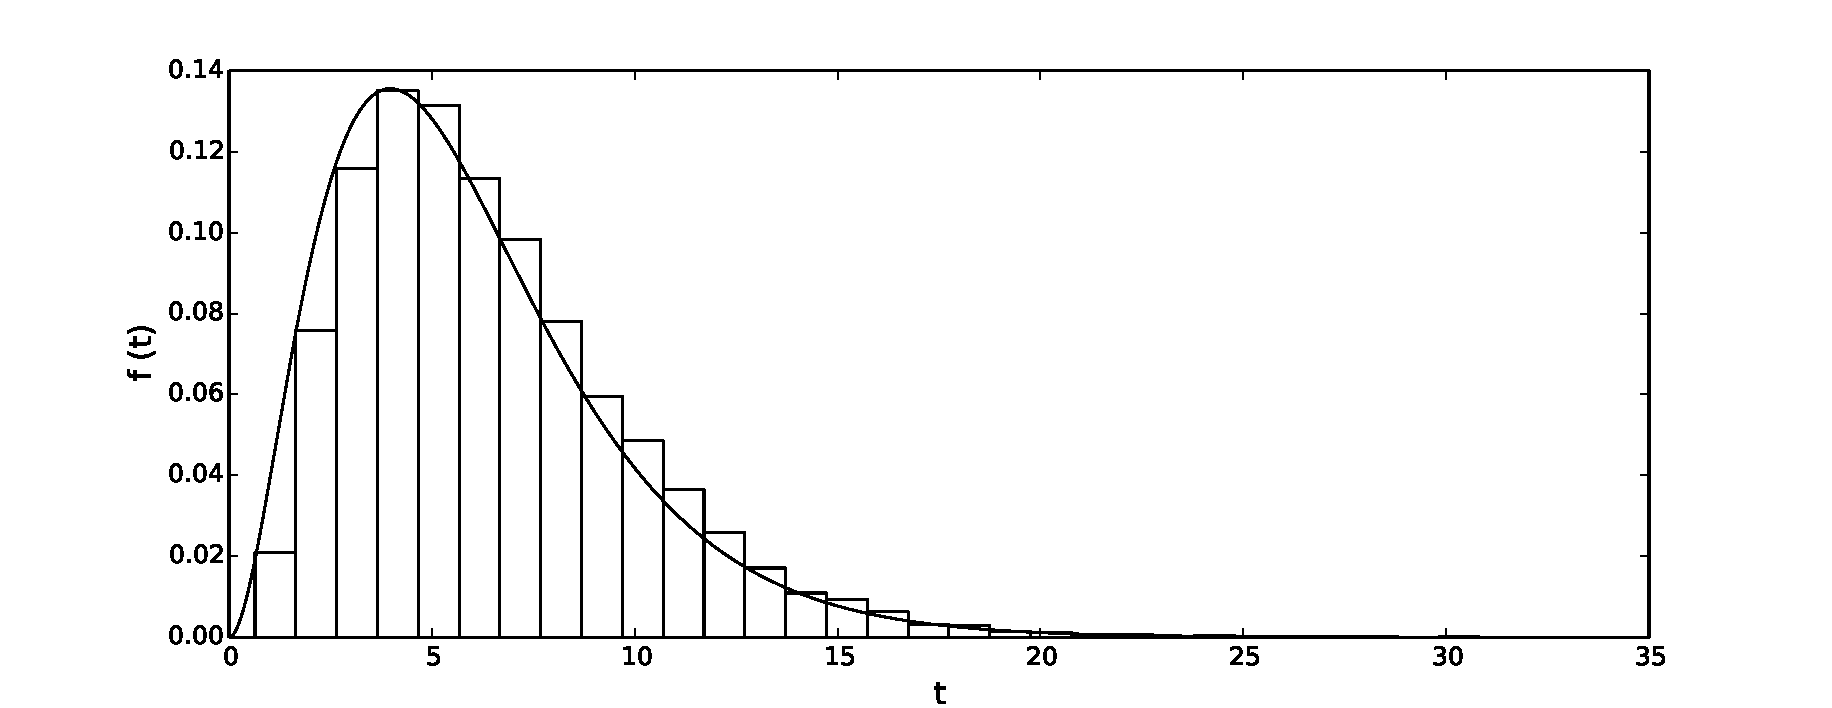
\includegraphics[height=6cm]{figure_1.pdf}
    \caption{Example of a typical histogram method used to approximate a continuous gamma function in at discrete time bins}
\end{figure}

\noindent
The most straight-forward technique for information estimation is to
break up the domains of the variables of interest into partitions of
finite size referred to as ``bins", and approximate the respective
standard equation discretely, using the fractions of points falling
into these bins as local density estimates \cite{Kraskov}. This kind of
binning strategy can also be used for embedding spike trains into a
space: the temporal window of observation of neural activity is
subdivided into discrete time slices. Each of these bins can then
correspond a distinct dimension - as for example in the traditional
``direct" method proposed by Strong \textit{et al.} \cite{STRONG}.\\

\noindent
The problem with the above approach is that the bins must be very
narrow - down to a millisecond \cite{Victor-Reich} - in order to capture spike
timing with good precision. This requires estimation of a tremendous
amount of response probabilities as the number of possible spike
distributions increases exponentially with the model's resolution -
for example
$\approx 2.23 \times 10^{491}$ possible words over just a quarter of a
second at $1$ ms precision. As the bias of such estimates is roughly
proportional to the number of possibilities, it takes unrealistically
large amounts of sample data in order for them to be accurate
\cite{Victor.2002}. In fact, this is one of the main difficulties associated
with measuring information-theoretic quantities. Furthermore
high-dimensional spaces tend to be very sparse, which makes the issue
even worse.\\

\noindent
The data problem is generally addressed by \textit{non-parametric}
estimation methods.  The Kozachenko-Leonenko entropy estimator
\cite{Kozachenko-Leonenko} is one such method which addresses the issue for data taking
values in vector spaces. It is described as \textit{"a little-known
  asymptotically unbiased 'binless' estimator of differential
  entropy"} \cite{Victor.2002}. The basic idea behind this method is to use
$k$-nearest neighbour distance statistics to estimate local densities,
as first proposed in \cite{Dobrushin}. It has substantial computational
advantages for estimating the entropy of a continuous distribution in
a Euclidean vector space and is guaranteed to be unbiased in the limit
of infinite sample data \cite{Kozachenko-Leonenko}. In \cite{Victor.2002} the
Kozachenko-Leonenko method is adopted for the estimation of the rate
of transmitted information through a neural "channel", which depends
on entropy estimation. In this paper however a dimensionality
assumption is made, which is resolved through a rather unnatural
foliation of the space of spike trains - it is split into two
components: a continuous one representing spike timing and a discrete
one expressing the number of spikes in a neural response. It is
demonstrated that for a limited-sized sample data the method
outperforms considerably traditional estimators relying on binning.\\

\noindent
Although this approach to entropy estimation dates back to
\cite{Dobrushin}, for a long time it had not been adapted to estimate
mutual information. A simple way to do this would be to make use of
the chain rule for entropy and the definition of mutual information:\\

\textit{Chain rule}
\begin{equation}
H(X,Y) = H(X) + H(Y|X) = H(Y) + H(X|Y)
\end{equation}

\textit{Mutual Information}
\begin{equation}
I(X;Y) = H(X) - H(X|Y) = H(Y) - H(Y|X)
\label{MI(X;Y)=H(X)-H(X|Y)}
\end{equation}

\noindent
From the above it follows that mutual information can be expressed as:
\begin{equation}
I(X;Y) = H(X) + H(Y) - H(X,Y)
\end{equation}

\noindent
The $k$-$th$ nearest neighbour estimator can be applied to individual
terms. However this could mean that statistical errors incur from all
individual entropy estimates. In \cite{Kraskov} two slightly different
algorithms both based on the ideas of Kozachenko and Leonenko are
given which deal with this issue and are shown to produce satisfactory
results. These however still depend on the dimensionality of the
variables and cannot be applied directly to the broader class of
metric spaces.\\

\noindent
Houghton and Tobin first propose a method for calculating mutual
information in metric spaces in \cite{Tobin-Houghton}. Here the kernel density
estimation technique (KDE) for approximating probability distributions
is adapted to estimate local densities on metric space data. The model
is motivated by the difficulty of estimating mutual information
between discrete stimuli and spike-train responses.\\

\noindent 
It is noticed that for large enough sample sets the KDE estimator
resembles a $k$-$th$ nearest neighbour estimator such as the one
proposed in \cite{Kraskov}. By using different values of $k$ in the
subspaces of each variable the terms depending on their
dimensionalities cancel. The method is tested against a histogram
approach, which essentially follows the binning strategy, on fictive
data, modelled to mimic the properties of spike trains and
electrophysiological data. It is shown that the KDE estimator
considerably outperforms the histogram approach as sample size and
dimensionality/number of "spikes" increase. The metric-space method's
estimation error is low and decreases as the amount of data grows, in
contrast to the binning one which retains a relatively high error rate
throughout.\\

\noindent
This leads to the model of interest, proposed by Houghton in
\cite{Houghton}, which builds on the results seen in \cite{Tobin-Houghton} and gives
a method for estimating mutual information in both the cases when one
variable is discrete and when both of the variables come from a metric
space. The derivation is more straight-forward and intuitive - some of
the complications associated with the KDE technique are avoided 
and the terms dependent on dimensionality in the $k$-$th$ nearest
neighbour estimator introduced in \cite{Kraskov} are avoided. In addition
a formula is derived for estimating the Kullback-Leibler divergence
between two probability distributions in the same metric space.\\


\addcontentsline{toc}{subsubsection}{The proposed model: probability as a measure in open balls}
\subsubsection*{The proposed model: probability as a measure in open balls}
\noindent
The lack of coordinates necessitates the introduction of an
alternative strategy for measuring volumes in a metric space. The
basic idea in \cite{Houghton} is that if $\mathcal{X}$ is a metric space
it is possible to measure the distance $d(x,y)$ between any two points
$x$ and $y$ and it is therefore possible to define a region, or
\textit{open ball}, $B_{\epsilon}$ around a point $x_i$ such that

\begin{equation}
B_{\epsilon}=\{ t \in \mathcal{X}: d(x,t) <\epsilon \}.
\end{equation}

\noindent
The volume $V$ of the ball can then be estimated from the marginal probability mass contained in it - that is %<-i.e. 
by counting the number of %<-
sample points it contains.\\

\noindent
The probability that such a region contains exactly $k$ out of $N$ possible sample points is given by the binomial distribution:

\begin{equation}
P_k(x_i) = \binom{N}{k}F_i^k(1-F_i)^{N-k}
\label{binom.k.no.pts}
\end{equation}

\noindent
Here $F_i$ is the probability mass contained in region $B$. If we
assume that the probability mass function is constant within the
region, then it can be approximated by

\begin{equation} 
F_i \approx Vp_X(x_i).
\end{equation}

\begin{figure}[H]
	\centering
	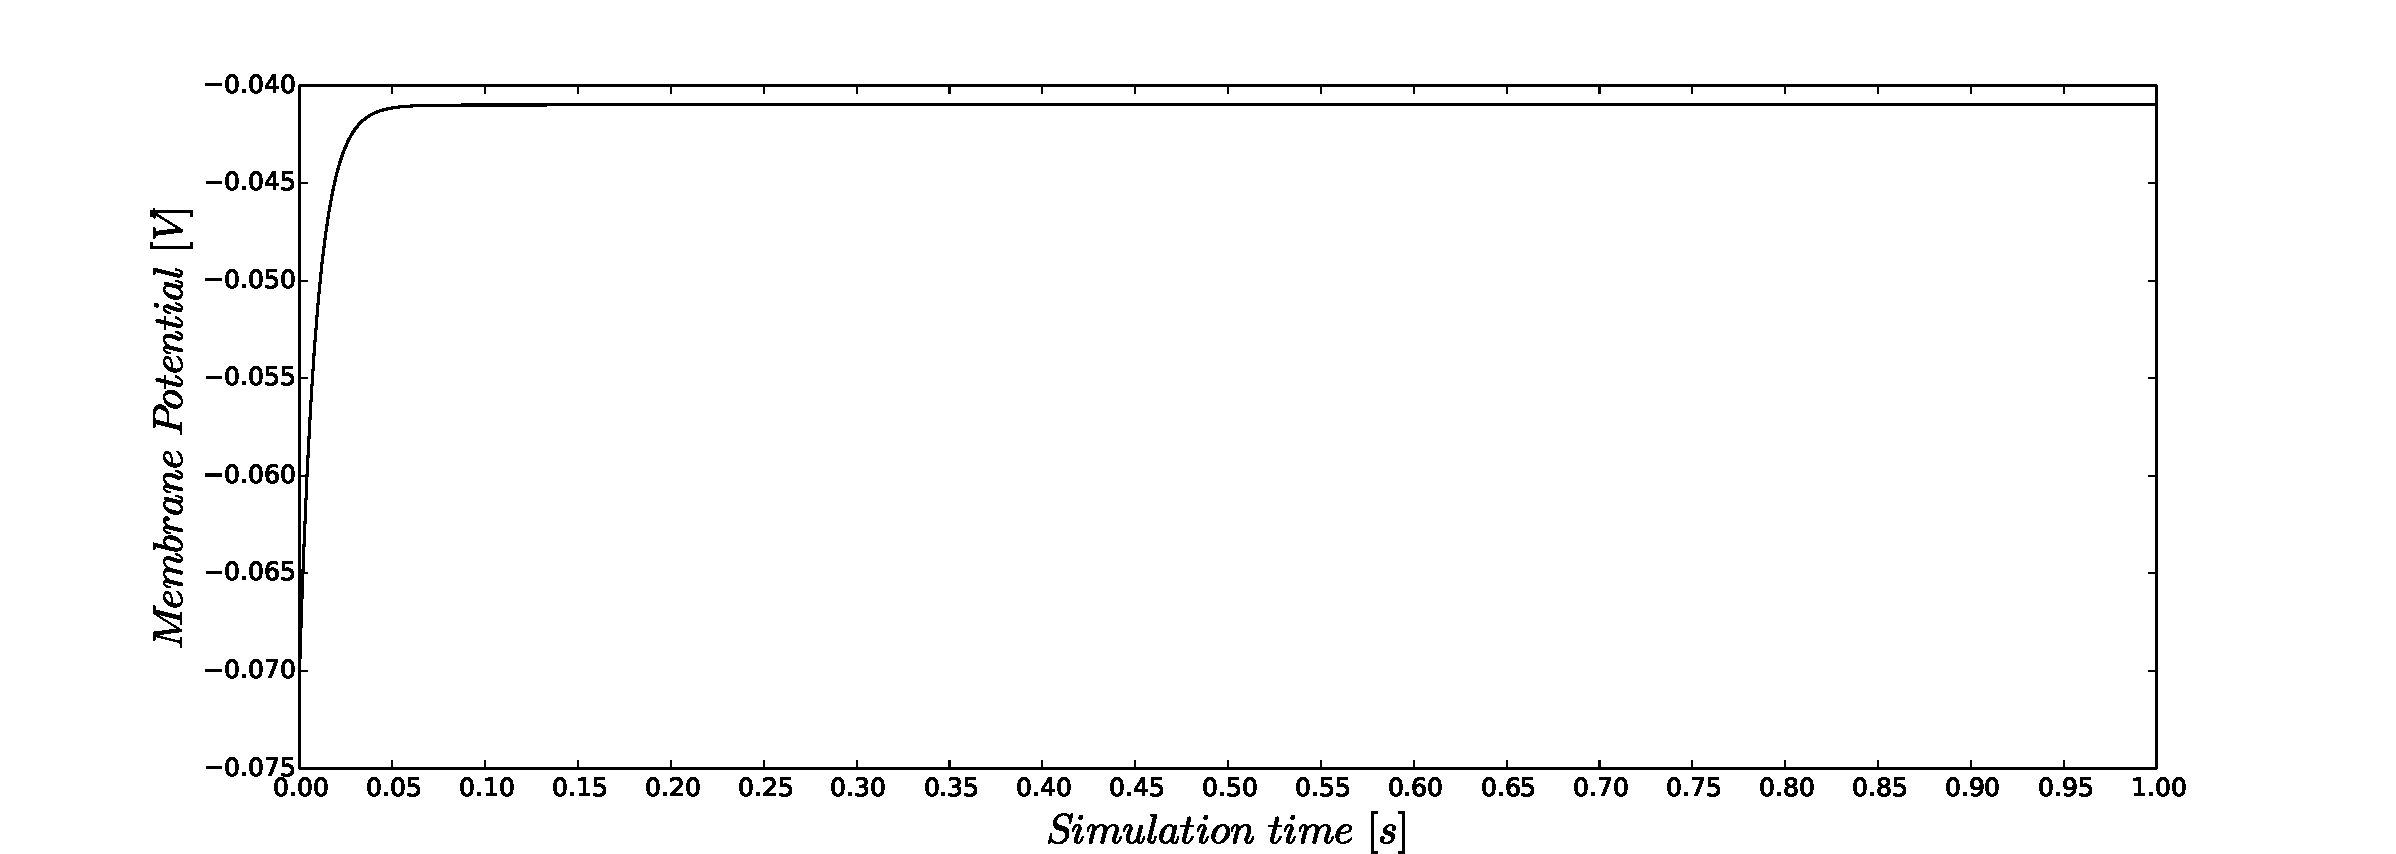
\includegraphics[height=9cm]{figure_2.pdf}
    \caption{Open ball around of radius $\epsilon$ around instanse $x_i$ in metric space $\mathcal{X}$.}
\end{figure}

\noindent
The justification for this is that variation in $p_X(x_i)$ should be
negligible for the purposes of this approximation as long as the ball
$B$ is small enough. The same assumption underlies the models in
\cite{Kozachenko-Leonenko,Kraskov}. On the other hand, the expected number of points in
the region is given by

\begin{equation}
\langle k \rangle = NF_i.
\label{eq.<k>=NF_i}
\end{equation}

\noindent
Letting $\#[B]$ denote the number of points in region $B$ as estimated from the data, from the above it follows that

\begin{equation} 
NVp_X(x_i) \approx \#[B(x_i,V)].
\label{prob.approx.eq}
\end{equation}

\noindent
Expressing equation \ref{eq.entropy.1} for a finite sample set of size $N$ as 

\begin{equation}
H(X)=-\frac{1}{N}\sum_{i = 1}^{N} \log_2 p_X(x_i)
\end{equation}
and using the above approximation to estimate 

\begin{equation}
\log_2 p_X(x_i) \approx \log_2 \frac{\#[B(x_i,V)]}{NV}
\end{equation}
the entropy of a random variable $X$ in metric space, using region-based
local density estimates, can be given as

\begin{equation}
H(X) \approx \log_2N + \log_2V - \frac{1}{N} \sum_{i = 1}^{N} \log_2\#[B(x_i,V)].
\end{equation}
This formula is similar to the ones proposed in \cite{Kozachenko-Leonenko,Kraskov} but it
is simpler. The main difference is that the probability is estimated
using the expected number of points in a region rather than the size
of the ball containing a given number of points in a coordinate
space. This approach is taken in order to avoid quantities that depend
on integrable manifolds.\\

\noindent
Nonetheless a way to measure the volume of the region is needed. Since there
is no obvious measure on a metric space without coordinates, it can be
defined in terms of the probability distribution estimated from the
data as the fraction of points falling in the region:

\begin{equation}
V\approx \frac{\#[B]}{N}.
\label{eq.vol.est}
\end{equation}

\noindent
Using such a measure, together with the above approximation for
$p_X(x)$, the probability would always equal one and therefore it
would always give a trivial estimate of entropy equal to zero.
Probability cannot be used as a measure to estimate the
entropy of a single random variable as it becomes self-referential.
Furthermore the entropy of a variable depends strictly on the measure
used in the domain of the variable. Mutual information however is not
measure-dependent and it involves more than one variable. Therefore
one probability distribution can be used as a measure for estimating
others. This is the key idea underlying the suggested model.\\

\noindent
In \cite{Houghton} two cases are considered reflecting two types of
neuroscientific experiments. In the first, one of the variables is
discrete, representing the stimulus - for example the location of a 
laboratory mouse on a 2D arena, and the other one
takes values in a metric space - such as a spike train in the space of
a similarity metric. In the second one, both random variables take
values in metric spaces.\\

\noindent
First the case when one variable is discrete is introduced. Given a
discrete set of stimuli $\mathcal{S}$ of size $|\mathcal{S}|=n_s$,
each presented exactly $n_t$ times (for simplicity), a total number of
$N=n_sn_t$ spike-train responses from a set $\mathcal{R}$ are
elicited. Using a similarity metric on the space of spike trains,
regions around each sample point are defined with $\epsilon$ chosen
such that they contain exactly $h$ neighbouring samples,
that is $V=h/N$. With the total probability, $p_R(r)$ used as a measure,
the entropy equals zero as seen before, but it can be used for
defining an estimate of conditional entropy, based on the conditioned
probability:

\begin{equation}
p_{R|S=s}(r) \approx \frac{\#[B]}{n_tV}.
\label{prob.approx.eq.2}
\end{equation}
This is analogous to the approximation from equation \ref{prob.approx.eq}
The entropy of $R$, conditioned on stimulus $s$ is then estimated by

\begin{equation}
\begin{aligned}
H(R|S=s) &\approx - \frac{1}{n_t} \sum_{i=1}^{n_t} \log_2 \frac{\#[B(r_i, V)]}{n_tV} \\
         &\approx - \frac{1}{n_t} \sum_{i=1}^{n_t} \log_2 \frac{n_s\#[B(r_i, h/N)]}{h}
\end{aligned}
\end{equation}
Averaging over $s \in \mathcal{S}$ as in the equation for conditional entropy 
(eq. \ref{eq.cond.entropy}) this gives

\begin{equation}
H(R|S) \approx - \frac{1}{N} \sum_{i=1}^{N} \log_2 \frac{n_s\#[B(r_i, V)]}{h}.
\end{equation}
Using equation \ref{MI(X;Y)=H(X)-H(X|Y)} the mutual between $R$ and $S$ information is derived as

\begin{equation}
I(R;S) \approx \frac{1}{N} \sum_{i=1}^{N} \log_2 \frac{n_s\#[B(r_i, V)]}{h}
\end{equation}
since $H(R)=0$ using the same measure.\\

\noindent
In the case where both variables $S$ and $R$ take values in metric
spaces the probability mass functions $p_S(s)$ and $p_R(r)$ are used
to measure volumes in $\mathcal{S}$ and $\mathcal{R}$ resulting in
entropy estimates equal to zero. But these measures induce a measure
on $\mathcal{S} \times \mathcal{R}$, which is the space where
stimulus-response sample points live. A region, or \textit{square}, in
$\mathcal{S} \times \mathcal{R}$ is then defined as the cross-section
of open balls in $\mathcal{S}$ and $\mathcal{R}$:

\begin{equation}
S\left( s_i, r_i, \frac{h_1}{N}, \frac{h_2}{N} \right) = \left\{ (s,r) \in \mathcal{S} \times \mathcal{R} : s \in B_S\left(s_i, \frac{h_1}{N}\right), r \in B_R\left(r_i, \frac{h_2}{N}\right)\right\},
\end{equation}
that is the set of stimulus-response pairs where $s$ is one of the
$h_1$ nearest neighbours of $s_i$ and $r$ is one of the $h_2$ nearest
neighbours of $r_i$.\\

\noindent
Under this new measure the volume of the region is

\begin{equation}
\textnormal{vol } S\left( s_i, r_i, \frac{h_1}{N}, \frac{h_2}{N} \right) = \textnormal{vol } B_S\left(s_i, \frac{h_1}{N}\right) \cdot \textnormal{vol }B_R\left(r_i, \frac{h_2}{N}\right) \approx \frac{h_1h_2}{N^2}.
\end{equation}

\noindent
And thus the mutual information is estimated by

\begin{equation}
I(R;S) \approx \frac{1}{N} \sum_{i=1}^{N} \log_2 \frac{N\#[S(s_i,r_i, h_1/N,h_2/N)]}{h_1h_2}.
\label{eq.MI.2x.metric}
\end{equation}

\noindent
The resolution of this model given by the $h_1$ and $h_2$ parameters
needs to be chosen appropriately. If they are too large the
approximation given in equation \ref{eq.<k>=NF_i} becomes less accurate due to the
assumption that probability mass function is constant in the ball. If
they are made too small on the other hand the accuracy of estimates in
equations \ref{prob.approx.eq} and \ref{prob.approx.eq.2}, where the mean value is estimated by
counting, is decreased.\\

\noindent
It is important to note that when the two variables are independent
the above equation gives an estimate of zero as required by the
definition of mutual information. This is because there is a
probability equal to $h_1/N$ for each of the $h_2$ points in $B_R(r_i,
h_2/N)$ to be also in $B_S(s_i, h_1/N)$ which means that there are on
average $h_1h_2/N$ points in $S(s_i,r_i,h_1/N,h_2/N)$, giving a
probability estimate of one.\\

\begin{figure}[H]
	\centering
	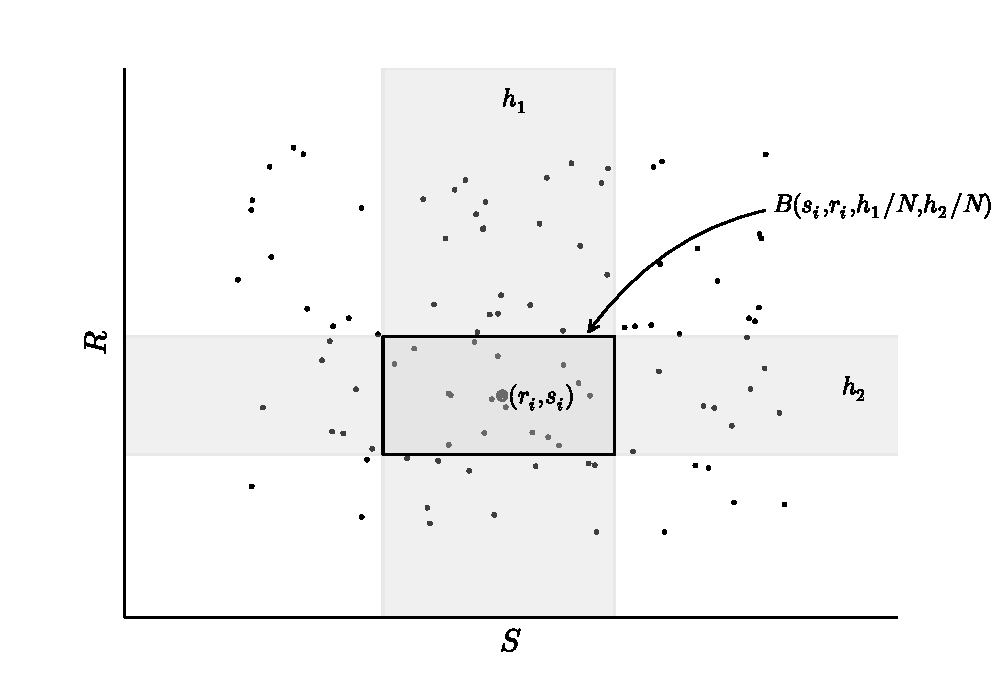
\includegraphics[height=9cm]{figure_3.pdf}
    \caption{Probabilities are estimated in $\mathcal{S}\times\mathcal{R}$ by counting the data points in region $B$, which is the cross-section of the balls around $s_i$ of volume $\frac{h_1}{N}$ and around $r_i$ of size $\frac{h_2}{N}$.}
\end{figure}

\noindent
The same approach is applied to estimate the Kullback-Leibler
diversion between the probability distributions of two random
variables taking values in the same metric space. This time however
the distribution of the second variable is used as a measure of the
volume of the regions around instances of the first one. That is if
$M$ instances are sampled from $R$ and $N$ - from $S$, then

\begin{equation}
\begin{aligned}
d(R||S) &\approx \frac{1}{M} \sum_{i=1}^{M} \log_2 \frac{p_R(r_i)}{p_S(r_i)}\\
		&\approx \frac{1}{M} \sum_{i=1}^{M} \log_2 \frac{N\#[B(r_i,h/N]}{Mh}
\end{aligned}
\label{eq.KL-dist.metric}
\end{equation}
where $B$ contains the $h$ instances sampled from $S$ that are closest to $r_i$ and $\#[B]$ gives the number of points sampled from $R$ falling in the ball.
Measuring the Kullback-Leibler divergence between the joint and product
distributions of $(s,r)$ pairs in a metric space $\mathcal{X}^2$ in
turn reduces to the formula for mutual information: setting the volume
to $h_1h_2/N^2$ for $N$ samples, equation \ref{eq.KL-dist.metric} reduces to equation
\ref{eq.MI.2x.metric}.\\

\noindent
The model aims to show that the Kozachenko-Leonenko approach for
information estimation can be applied in this simple form to sample
spaces without coordinates. The problem that inspires it arises from
the difficulty of estimating information on electrophysiological data
embedded in high-dimensional Euclidean spaces, 
but it can be applied to a much broader range of context. If
successful it could provide a framework for calculating information
shared between any variables taking values in a space where a suitable
similarity metric is defined. In the next part of this section the
problem of assigning distance between spike trains is discussed and
two state-of-the art solutions currently available are presented.\\

\addcontentsline{toc}{subsubsection}{Spike-train metrics}
\subsubsection*{Spike-train metrics}
\noindent
Being able to compare neural activity patterns over time and across a
population of neurons is of fundamental importance to understanding
the semantics of neural signalling. The spike-train metrics described
in \cite{Houghton-Victor} provide a principled approach to the problem. First,
two methods for comparing pairs of spike trains from single neurons
are introduced, which are then extended to the comparison of
spatio-temporal patterns of population activity. The aim is to
construct a mathematical framework for analysing neural coding - both
in terms of firing rates and precise spike timing.\\

\noindent
%this paragraph is confusing, it doesn't say what Euclidean space
The basic idea is to start with a very general geometric description
of the space of spike trains, thereby allowing for it to reflect their
specific physiological properties and avoiding fitting them to an
arbitrary standard which may not be suitable. Indeed, although
Euclidean vector spaces have proven to be very useful in many cases,
spike trains do not seem to comply with their rules. If every dimension
represents a spike time for example, similar spike
trains with different number of spikes would have to be parametrized
in different-dimensional spaces. There is also no natural way for
subtracting one spike train from another and no physiological
motivation for assuming that ``adding" the same spike train to two
spike trains preserves the distance between them. This is why the
space of spike trains is simply considered to be a metric space - one
where distances between points can be measured.\\

\noindent
Having said this, the first family of distances considered -
the van Rossum kernel-based metrics \cite{van.Rossum}, first map spike trains
into a vector space of functions and then use Euclidean distance to calculate
the distance between them. This method however avoids using a binning
strategy to embed a spike train into a discrete vector space with
dimensionality given by spike-count or the number of bins. Instead, it
maps a spike-train to a continuous function by convolving it with a
linear filter. This allows for the distance to be calculated directly
using the $L_2$-norm metric for functions. And although if computed numerically this 
has the structure of Euclidean distance in high-dimensional discrete vector 
space, such a space does not ever need to be used explicitly. The distance can be
solved analytically and taken as is, to form a metric space of spike trains.\\

\noindent
Here the van Rossum metric with an exponential kernel is
considered. This filter mimics the synaptic conductance dynamics
resulting from a spike. It expresses the idea that the distance
between spike trains should reflect the difference in their effect on
other neurons by drawing a caricature of the effect of a spike on
membrane potential.\\

\noindent
A spike train $\mathbf{u} = \{u_1, u_2, \ldots, u_m\}$ is mapped to a real function using a kernel $h(t)$:

\begin{equation}
\mathbf{u} \mapsto f(t; \mathbf{u}) = \sum_{i=1}^{m} h(t - u_i),
\end{equation}
the kernel itself is defined as 

\begin{equation}
h(t) = \begin{cases}
    0, & t<0\\
    \frac{1}{\tau} e^{-t/\tau}, & t \geq 0
  \end{cases}
\end{equation}
where $\tau$ is a time scale associated with the synapse. The distance
between spike trains $\mathbf{u}$ and $\mathbf{v}$ is given by the
$L_2$ distance between the corresponding functions:

\begin{equation}
d(\mathbf{u}, \mathbf{v}; \tau) = \sqrt[]{\int dt[f(t;\mathbf{u}) - f(t;\mathbf{v})]^2}
\end{equation}
For the causal exponential filter this integral can be solved analytically \cite{Houghton-Kreuz.12} to express the distance as a summation in terms of exponentials:
\begin{equation}
d(\mathbf{u}, \mathbf{v}; \tau) = \sqrt[]{\sum_{i,j} e^{-|u_i-u_j|/\tau} + \sum_{i,j} e^{-|v_i-v_j|/\tau} -2\sum_{i,j} e^{-|u_i-v_j|/\tau} }. 
\end{equation}


\noindent
When an action potential arrives at a synapse it causes an abrupt
rise in the conductance of the post-synaptic membrane. Eventually this 
results in a spike in the membrane potential of the post-synaptic
neuron. This event occurs on a time scale much smaller than the rest
of neural electrodynamics, which is why it is modelled as
instantaneous:

\begin{equation}
f \rightarrow f + \delta f.
\end{equation}

\noindent
The increment $\delta f$ depends on the scale chosen - it can be set to one. 
After the spike has arrived the conductance is assumed to drop at a constant rate

\begin{equation}
\tau \frac{d}{dt}f = - f
\end{equation}
hence the exponential decay. This construct can incorporate another
aspect of synaptic conductance - its dynamics when multiple spikes
arrive within a short time interval. Since there is a great variety of
synapses, the limit to their conductance is variable too. In many
synapses the arrival of a spike has a diminishing effect on subsequent
impulses arriving shortly after it. This can be modelled by adding an
extra parameter but will not be discussed here as it is not necessary
for the purposes of this project.\\

\noindent
The other family of spike-train distances is the one of edit-length
metrics, exemplified by the Victor-Purpura metric \cite{Victor-Purpura_1,
  Victor-Purpura_2}. As mentioned above this is similar in spirit to the Hamming
distance used in string matching. In particular, it defines the
distance between two sequences of spikes as the cost of moulding one
into the other. As a result, no intermediate representation is
required but rather the distance can be computed immediately given a
pair of spike trains.\\

\begin{comment}
This can be modelled by adding an extra parameter:
\begin{equation}
	\delta f = 1 - \mu f
\end{equation}
with $0 \leq \mu \leq 1$. When $\mu$ is equal to zero, the function
increases by a unit at every spike as in the original kernel map,
expressing an unlimited capacity of the synapse to conduct
current. When it is non-zero on the other hand, $\mu$ scales the
function at the arrival of an impulse depending on its immediate
history, reflecting a short-term ``depressing'' effect of a spike on
synaptic conductance. The effect of this extra parameter on the
distance measure is that some spikes contribute a greater amount to it
than others, depending on how closely they follow previous spikes. Due
to the interaction between spikes occurring at different times the
mapping cannot be thought of as a linear filter when used with this
extension - it can rather be represented as a sum of non-linear
kennels of increasing order.
\end{comment}

% maybe add the squared function to the plot to illustrate the
% volume of the distance
\begin{figure}[H]
	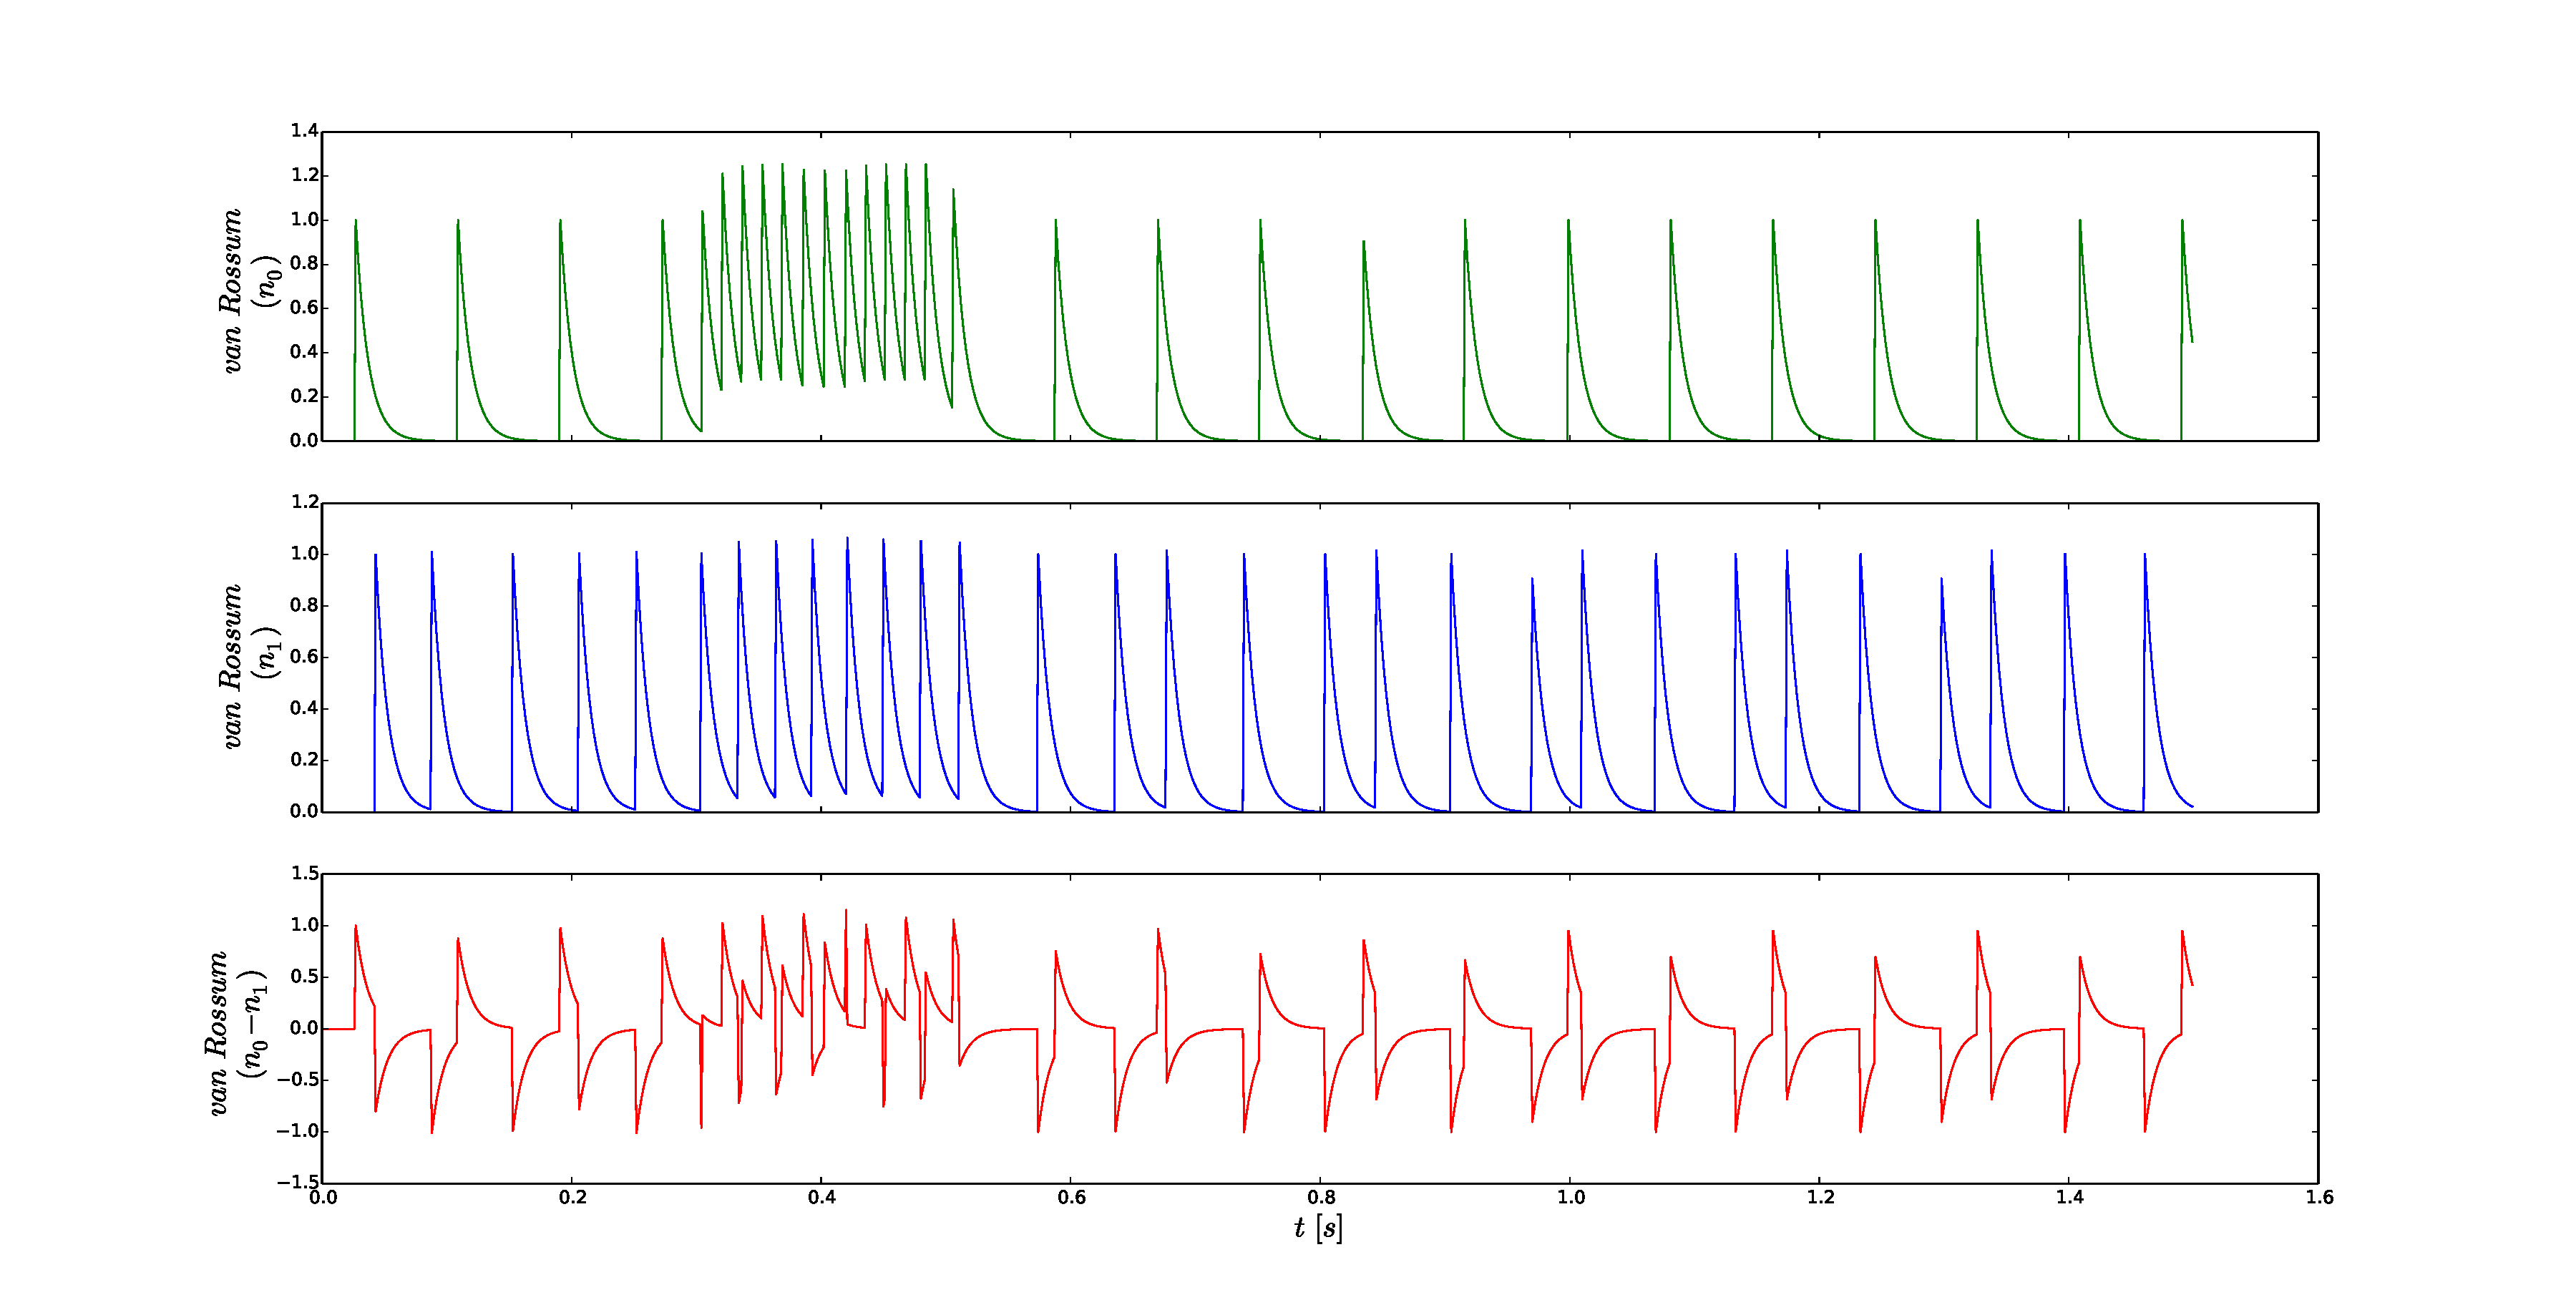
\includegraphics[height=9cm]{van_Rossum_difference.pdf}
    \caption{(top, middle) Mapping spike trains to functions using the 
 van Rossum metric with an exponential kernel. (bottom) Subtracting one
 function from the other.}
\end{figure}

\noindent
The main concept associated with an edit-distance is a \textit{cost
  function} defined in terms of a set of \textit{elementary steps},
each assigned a non-negative individual cost. In the context of
strings of symbols over a finite alphabet this usually includes the
three basic operations - insertion, deletion and substitution. The
total cost $c(\gamma)$ of transforming one sequence into another is
thus given by the set of elementary steps that can be used to complete
the task at a minimal overall cost:

\begin{equation}
d(\mathbf{u},\mathbf{v}) = \min_{\gamma} c(\gamma)
\end{equation}

\noindent
As long as the cost of a step equals the cost of inverting it this
distance is certainly symmetric. For the purposes of comparing spike
trains, the basic elementary step consists of inserting or deleting a
spike and has a unit cost, which sets a scale on the metric. This
guarantees there is a finite distance between any pair of spike trains
given by replacing all spikes from one train with the spikes of
another one, and equal to the sum of their lengths. In the simple case
of the Victor-Purpura ``spike-time'' metric, a second elementary step
is added consisting of moving a spike by some amount of $\delta
t$. This step has a cost of $q\delta t$ associated with it, where the
parameter $q$ determines the cost per distance for moving a
spike. This means that the cost of moving a spike cannot exceed the
cost of deleting it and inserting a new one at the desired position in
time: $q\delta t < 2$, so the maximum distance by which any spike can
be moved to achieve minimum total cost is given by a time-scale of
$2/q$ determining the sensitivity of the metric.\\

\noindent
The problem of finding an optimal sequence of steps can addressed
efficiently using a dynamic programming procedure:\\

\begin{algorithm}[H]
  \KwIn{spike trains $\mathbf{u}$ of length $m$, $\mathbf{v}$ of length $n$}
  \KwOut{$d(\mathbf{u},\mathbf{v}) = \min_{\gamma} c(\gamma)$}
  $G \leftarrow$ array of size $m\times n $\\
  $G_{i,0}\leftarrow i$ $\mathbf{for}$ $i \in \left[1,m\right]$, $G_{0,j}\leftarrow j$ $\mathbf{for}$ $j \in \left[1,n\right]$\\
  \For{$i\leftarrow 2$ \KwTo $m$}{
    \For{$j\leftarrow 2$ \KwTo $n$}{
      $G_{i,j} \leftarrow min(G_{i-1,j-1} + q|\mathbf{u}_i-\mathbf{v}_j|, G_{i-1,j}+1, G{i,j-1}+1)$ \\
    }
  }
  \KwRet $G_{m,n}$\\
   \vspace{11pt} \caption{Matching one spike-train to another at minimum cost}
\end{algorithm}
\vspace{16pt}

\noindent
The above algorithm takes advantage of the properties of minimum
cost-sequences which exclude inefficient steps such as moving a spike
from one train past a spike from the other, or making redundant moves
in combination with insertions or deletions. Every entry $G_{i,j}$
denotes the distance between the sub-trains containing the first $i$
spikes from $\mathbf{u}$ and the first $j$ spikes from
$\mathbf{v}$. At each step, the algorithm considers the last spikes
from the respective sub-trains and makes a minimum-cost choice among
three possibilities: 1) matching the two spike trains, 2) deleting the
last spike from one train, or 3) inserting a new spike into it
matching the last one of the other. In this way the dynamic
programming paradigm is applied - avoiding recursion by storing the
results from previous computations and building the final result from
the bottom up.\\

%again, not clear you need all of this, just one paragraph on extensions would do
\noindent
Both the kernel-based van Rossum metric and the edit-length
Victor-Purpura metrics can be extended to compare population activity
by extending the domain in which spikes occur with another variable
apart from time - the ``neuron of origin''. This involves adapting
each of them in specific ways reflecting their mathematical
properties, but abstracting away from these details an important
parallel can be drawn between multi neuronal metrics and another
similarity measure used in image analysis - the\textit{ Earth Mover
  Distance} \cite{Rubner.Earth-mover}. The concept is that an image, 
represented by a histogram is thought of as a 3D terrain, and
the similarity between it and another image is measured in terms of
the labour - volume$\times$distance, required to match one terrain to
the other. In order to do so a cost function is
defined consisting of elementary steps for moving adding and subtracting
mass. This approach can in turn be extended to incorporate
higher-dimensional objects such as video, volumetric images or
functional data. The cost for moving events does not need to be
dimension-invariant in any of these cases nor does it need to reflect
Euclidean distances. This example aims to show that alternative
metrics can be used in many contexts and methods for estimating
probability and information quantities in the spaces they give rise to
can be useful to various applications.\\

\noindent
The two types of spike-train similarity measures described above have
very different mathematical structures but they are both quite
successful in capturing the differences between neural activities in
terms of their effects on other neurons. One of the ways this is
tested and verified is by examining their performance when used to
cluster together spike trains elicited in response to the same
stimulus. Interestingly, regardless of their distinct properties the
kernel-based and edit-length metrics perform very similarly on this
task. This can be explained by noting that under certain settings the
metrics themselves treat spike trains in an analogous fashion. These
will not be discussed here - instead the variants introduced will both
be used to test the information estimator in order to verify its
validity and test its performance in metric spaces with varied
underlying structure.\\

\noindent
The next and final section of this chapter explores the general
physiological properties of nerve cells and the mechanisms they use to
connect and interact in the nervous system, along with the
mathematical models used to describe them relevant to this project. It
does not aim to encompass the full picture of their neurological
understanding, but rather to motivate the computational model used to
implement a simulation of a network of spiking neurons in
software. This network will serve as the basis of an environment for
configuring experiments that generate spike-train data which will be
used to test the mutual information estimator.\\

\newpage
\subsection{Scientific and technical aspects}

\begin{figure}[H]
	\centering
	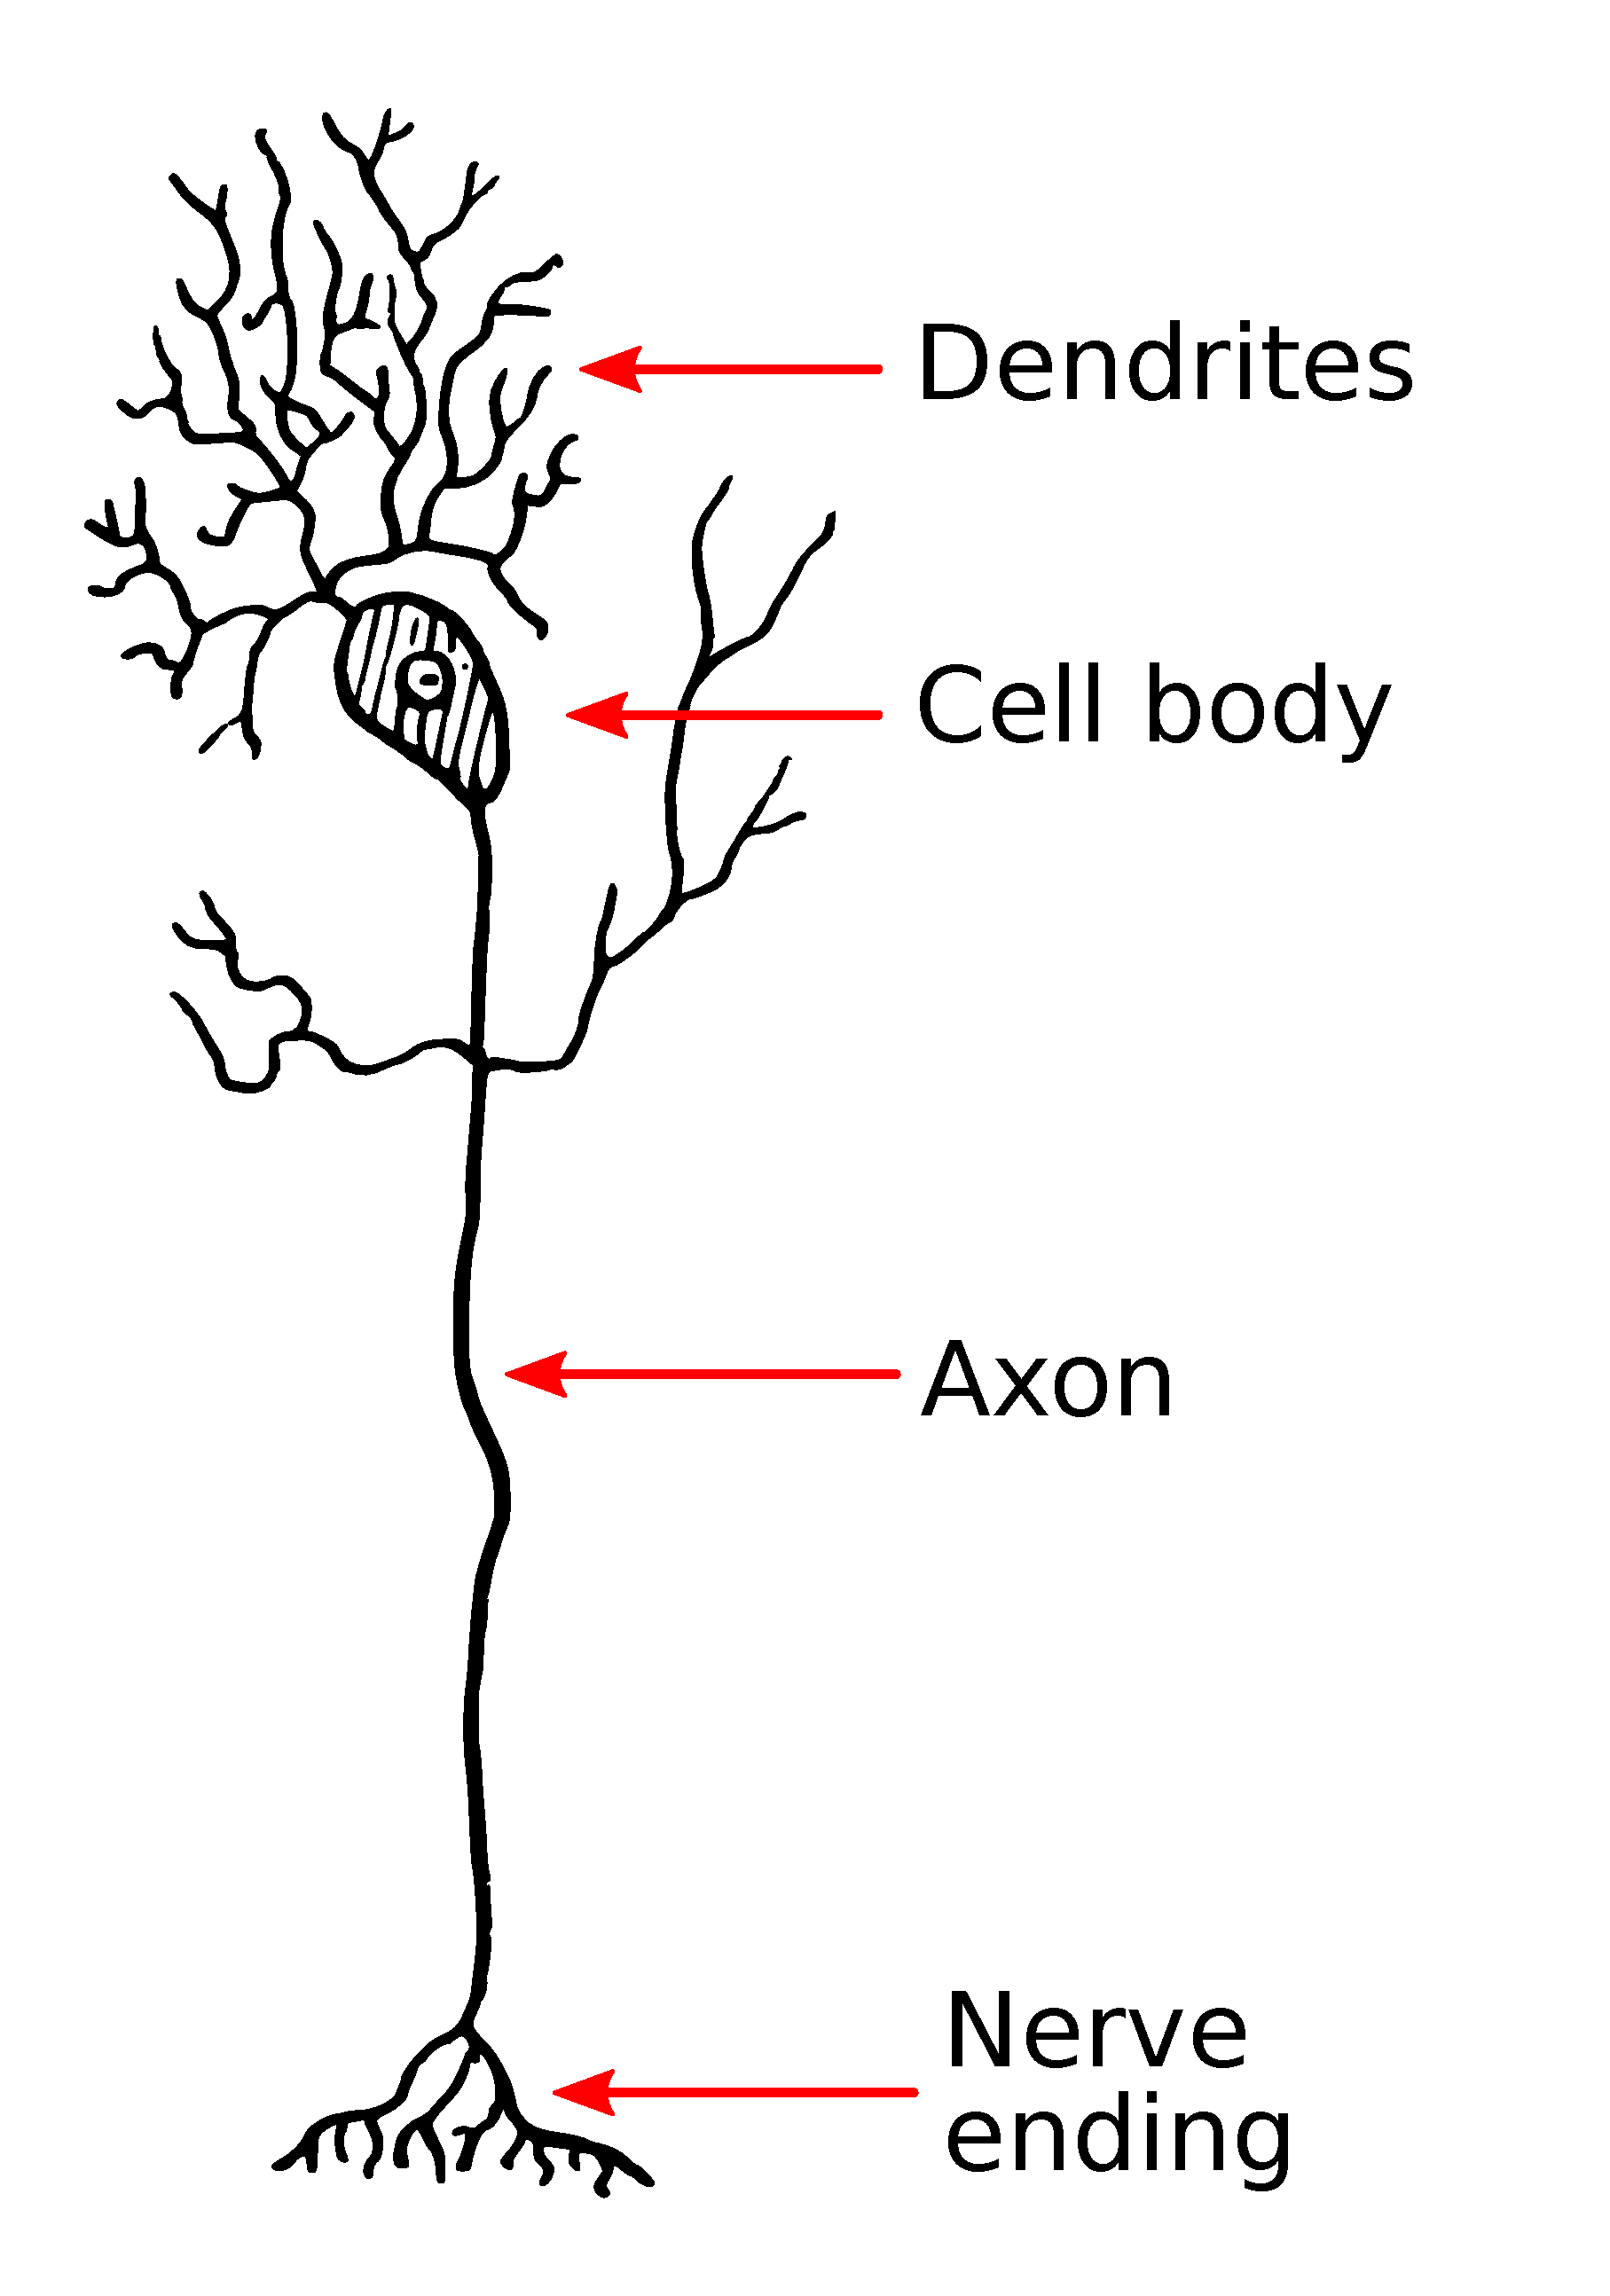
\includegraphics[height=8cm]{neuron.pdf}
    \caption{Simple diagram of a neuron from \href{https://commons.wikimedia.org/wiki/File:Dendrite_(PSF).svg}{\underline{Wikimedia Commons}}.}
\end{figure}

\addcontentsline{toc}{subsubsection}{The nerve cell}
\subsubsection*{The nerve cell}
\noindent
The nerve cell, or \textit{neuron}, is arguably one of the most
interesting and important cells found in the bodies of nearly all
animals. It is absent only in a few very simple multicellular
organisms such as sponges. Together with the \textit{glial} cells
(Greek for glue), which support them structurally and metabolically,
they constitute the nervous systems that govern the activity of
organisms. This is accomplished through the communication and
processing of information in the form of electrical signals
transmitted between neurons connected in networks.\\

\noindent
Morphologically the neuron can be seen as being comprised of three
main components. Through the \textit{dendrites}, signals are received
by the cell body, or \textit{soma}, which processes them and in turn
transmits a signal along the \textit{axon} reaching out of it towards
other cells. The characterising property of neurons is that they are
electrically excitable by other neurons. Most commonly, they connect
to each other via chemical synapses mediating electrical charges
between their axons and dendrites. In this context neurons are
distinguished as pre-synaptic and post-synaptic. There are two types
of synapses: excitatory - making the post-synaptic neuron more likely
to signal, and inhibitory - suppressing its signalling.\\

\noindent
An electric impulse is elicited by the nerve cell when the potential
difference across its membrane exceeds a certain threshold - typically
around $-55$ mV. When the cell is at rest, the electric potential
inside is lower than the potential outside of it. The potential
difference is referred to as \textit{membrane potential}, amounting to
about $-70$ mV when at ease. This state is actively maintained by
\textit{ion pumps} - mechanised protein channels moving electrically
charged particles across the membrane of the cell using energy. An
ubiquitous example is the sodium-potassium adenosine triphosphatase
enzyme. It pumps three positively charged sodium (Na+) ions out of the
cell for every two positive potassium (K+) ions it pumps inwards,
resulting in a loss of one atomic charge per pumping cycle. In this
way potassium is concentrated inside the soma whereas sodium is pushed
out. The negative voltage equilibrium is a result of this
saturation. The random thermal motion of potassium ions causes them to
diffuse outwards despite of the lower potential inside the cell body,
which on the other hand attracts sodium. It takes the reciprocal
activity of the ion pumps to counteract this force and compensate for
the leak of charge.\\

\noindent
A neuron can be either excitatory or inhibitory in the sense that as a
pre-synaptic neuron it can form either only excitatory or only
inhibitory synapses to other, post-synaptic neurons. Chemical synapses
work by virtue of the release of substances called
\textit{neurotransmitters} from the terminal of the axon of the
pre-synaptic neuron due to the arrival of an electrical impulse. The
released neurotransmitter fits like a key in a lock into binding sites
called \textit{receptors} situated in the dendrites of the
post-synaptic neuron. The receptors open up specialised
\textit{ligand-gated} ion channels and allow ions through the membrane
of the post-synaptic neuron for a short time period. Depending on the
type of the synapse and of the ion channels this leads to a small
increase or decrease in its membrane potential.\\

\noindent
When the voltage reaches its threshold value this activates the
opening of yet another type of ion channels allowing an abrupt influx
of sodium inside the cell during a narrow time window - $1$--$2$
ms. This produces a non-linear cascade in the membrane potential
called an \textit{action potential} or spike. This impulse then
propagates through the axon, being continuously amplified in the same
fashion by the opening and closing of voltage-gated channels along its
length.\\

\noindent
The story given here abstracts away many details important to an
accurate biological and physical description of the nerve cell and how
it works. Nevertheless it is sufficient to give an outline of the
behaviour of neural voltage dynamics for the purposes of the
mathematical model used to describe it introduced below.\\

\addcontentsline{toc}{subsubsection}{The leaky integrate and fire model}
\subsubsection*{The leaky integrate and fire model}

%I would define the integrate and fire neuron directly, rather than
%through the analogy of the bucket equations!

\noindent
In this project a variant of what is known as the leaky integrate and
fire model \cite{Lapique} is used to simulate the behaviour of spiking
neurons wired together in a network. This simplified model represents
the voltage dynamics of a neuron as a first-order ordinary
differential equation. An intuitive analogy can be made between this
equation and a similar one giving a simple model for the rate of
change in the height of water in a leaky bucket that is being
continuously filled from the top.\\

\noindent
The basic idea is that the rate $l$ at which water leaks out is
proportional to the height $h$ of the water inside the bucket as it
determines the pressure at its bottom. Assume for simplicity that $l$
also depends on a single constant $G$, reflecting the size of a hole
on the bottom and some other physical factors. The relationship
between the two is expressed as

\begin{equation}
l = Gh.
\end{equation}

\noindent
Let $i$ denote the rate at which water pours into the bucket and $C$ - the area of the base (the sides of the bucket are considered to be straight). The rate of change of the volume of water contained in the bucket is then

\begin{equation}
\frac{dCh}{dt} = i - Gh
\label{bucket.eq}
\end{equation}
and consequently the rate of change of its height is

\begin{equation}
\frac{dh}{dt} = \frac{1}{C}(i - Gh).
\end{equation}

\noindent
The height is used as an analogue for the voltage - greater height/voltage means greater difference in pressure/potential between the the two ends of the water-column/cell-membrane. In the model for the membrane potential the cross-sectional area of the bucket $C$ is replaced by the electric capacitance of the membrane $C_m$ and $G$ is substituted with $G_m$ - the conductance of the membrane. As mentioned above the equilibrium voltage at which there is zero current leaking through the membrane equals $-70$ mV and is actively maintained by the sodium-potassium pumps - this is called the \textit{reversal potential} of the membrane, denoted $E_L$. The leak current out of the cell is then given by Ohm's law as $G_m(V-E_L)$. Equation \ref{bucket.eq} is thus rewritten as

\begin{equation}
\frac{dC_mV}{dt} = I - G_m(V-E_L)
\end{equation}
where $I$ is the input current. In the original experiment by Lapicque \cite{Lapique} this is injected directly into the cell with an electrode - usually denoted $I_e$, but it could also stand for currents coming in through the synapses. Usually the equation is divided across by the conductance. The resistance is then denoted $R_m=1/G_m$ and $\tau_m=C_m/G_m$ gives a time scale for the membrane:

\begin{equation}
\tau_m\frac{dV}{dt} = E_L - V + R_mI.
\end{equation}

\noindent
This equation does not model the non-linear effect of the voltage reaching the threshold of about $-55$ mV which produces the spike. This is accounted for in a more detailed equation given by the Hodgkin Huxley model \cite{Hodgkin-Huxley} which includes terms for the currents due to the opening and closing of the voltage-gated channels. However, since the time-scale at which these non-linear dynamics occur is very narrow compared to the rest of the process, they can be modelled as occurring instantaneously. The equation will not be solved analytically but rather integrated numerically at discrete time steps in software using an approximation technique. Therefore a spike can be added by hand by setting the voltage to a value above zero once the threshold is reached and then immediately resetting it to to a value near the rest point of $-70$ mV. In fact, for the purposes of estimating information in spike trains, spikes will not even need be added but just recorded before $V$ is reset.\\

\noindent
The strategy described above for simulating neuronal activity numerically on a computer makes it easier to solve the model for a variable input current due to the synapses. The synaptic current is the last ingredient left to define in order to complete the model so that it can be used to simulate the dynamics of a population of integrate and fire neurons interacting together in a network. It will be modelled by the following equation

\begin{equation}
I_s(t) = g_ss(t)(E_s - V)
\end{equation}
where $E_s$ is the reversal potential of the synapse and $g_ss(t)$ is the conductance at the synapse - $g_s$ describes the synaptic strength and s(t) models the opening and closing of the ligand-gated channels due to the arrival of a spike: 

\begin{equation}
s(t) = G_{max}e^{-t/\tau_s}
\end{equation}
where $t_s$ is the time since the pre-synaptic neuron's last spike, $\tau_s$ is the time-scale of the synapse, and $G_{max}$ is a constant used to control the scale of the conductance. The exponential decay models the unbinding of neurotransmitter which closes the ligand-gated channels after they open. In a model that strives for accuracy $G_{max}$ can be replaced by $t$, but here it is assumed that the gates open instantaneously and the control parameter serves the purpose of tuning the simulation.\\

\noindent
The full equation for the voltage can now be given as

\begin{equation}
\tau_m\frac{dV}{dt} = E_L - V + R_mI_e + R_m\sum_{i=1}^{N}I_s(t,i)
\end{equation}
for a neuron with $N$ pre-synaptic neurons connected to it. The constant input current $I_e$ is optional and can be used to stimulate particular neurons or just to stabilise the network.\\


\addcontentsline{toc}{subsubsection}{Numerical methods}
\subsubsection*{Numerical methods}
\noindent
The technique used to compute a numerical solution to the membrane potential equation is known as the Runge-Kutta method \cite{Num.recepies.in.C}. It is based on the Taylor series expansion of a function around a point $t_0$:

\begin{equation}
f(t) = \sum_{i=0}^{\infty} \frac{1}{n!} \frac{d^nf}{dt^n}\biggr\rvert_{t=t_0} (t-t_0)^n.
\end{equation}

\noindent
This gives an iterative method for efficiently solving a differential equation of the form

\begin{equation}
\frac{df(t)}{dt} = F(f,t)
\end{equation}
to some approximation by expanding $f$ around discrete time-steps split by some small interval $\delta t$, up to a term of some order $N$. In other words $f(t+\delta t)$ can be worked out from $f(t)$ by using its derivative $F$:

\begin{equation}
f(t+\delta t) = f(t) + F(f,t)\delta t + \frac{1}{2}F'(f,t)\delta t^2 + O(\delta t^3).
\end{equation}

\noindent
The simplest way to go about this is to ignore the $\delta t^2$ and
smaller terms - this is known as the \textit{Euler method}. Sometimes
one might expect that the errors would have different signs and cancel
often enough to give a good approximation. However this is not always
the case - they might add and the $O(\delta t^2)$ error could cause a
considerable offset. The Runge-Kutta methods address this issue by
considering a number of different Taylor expansions so that the terms
$\delta t^2$ and smaller cancel. The most common version is the
classical Runge-Kutta fourth order method known as ``Num.recepies.in.C'':\\

Given an initial condition $f(t_0)$ let

\begin{equation}
\begin{aligned}
t_n &= t_0 + n\delta t \\
f_n &= f(t_n)
\end{aligned}
\end{equation}

then define the following four coefficients

\begin{equation}
\begin{aligned}
k_1 &= \delta t F(f_n,t_n) \\
k_2 &= \delta t F(f_n + k_1/2, t_n + \delta t /2) \\
k_3 &= \delta t F(f_n + k_2/2, t_n + \delta t /2) \\
k_4 &= \delta t F(f_n + k_3, t_n + \delta t)
\end{aligned}
\end{equation}

finally, compute the value of $f$ at time $t_{n+1}$ as

\begin{equation}
f_{n+1} = f_n  + \frac{1}{6}(k_1 + 2k_2 + 2k_3 + k_4).
\end{equation}

\noindent
The $k_i$ coefficients are increments based on estimates of the slope
of the function at different points through interval of length $\delta
t$. The weighted average of the four of them is taken ensuring the
error is $O(\delta t^5)$ without explicitly computing higher-order
derivatives of $f$. This approximation gives a considerable
performance improvement over the Euler method and gives good enough
precision for exploring neural voltage dynamics computationally.\\

\addcontentsline{toc}{subsubsection}{Poisson neurons}
\subsubsection*{Poisson neurons}

%This is confusing as you do it here, you have to explain that you are
%modelling neurons which are deterministic, as in the I&F neuron but
%are subject to background noise due to their rich connectivity,
%leading to stochastic behavior
%not sure how much of this material is relevant for what comes after!

In a real situation, timing between successful action potentials
elicited by neurons from many parts of the brain appears to be very
irregular under a wide variety of circumstances. It is even often
observed that spike trains produced in response to the same stimulus
over consecutive trials although similar would vary considerably both
in terms of their firing rates and spike times \cite{Dyan-Abbott}. Therefore it
is sometimes reasonable to model spiking as a stochastic process. In
the previous section a recipe for simulating a spiking neuron has been
introduced but such a neuron needs variable input in order to exhibit
interesting firing behaviour. Instead of constructing complex networks
or encoding this variability explicitly in the external stimulation
current, it is useful to be able to generate the spiking of some of
the neurons in a network as random sequences with some average firing
rate. In this way they can be used to provide input to others
simulated using the physiologically inspired model.\\

\noindent
In theoretical neuroscience the problem of estimating the probability
that a particular spike train occurs arises from the need to model the
relationship between a stimulus and a response. The total number of
possible spike sequences over a meaningful time interval is usually
excessively large so estimating the probability of each one is
infeasible. Therefore a statistical model based on a limited set of
observed responses is needed to estimate their probability
distribution. This is typically done in an attempt to predict the
stimulus that produced a given response or to quantify the probability
of the response itself occurring.\\

\noindent
Since spikes are considered to be stereotyped events proceeding at a
very tight time-scale they are idealised as occurring instantaneously
- an assumption that has been at work throughout this exposition by
the sheer use of spike trains. For a time bin, small enough to ensure
there can be no more than one spike occurring in it, the probability
of a spike can be determined by the firing rate of the neuron. This
statistic is generally not sufficient to predict the probability of a
spike train because because the joint probability of two spikes
occurring in particular time-slots is not necessary equal to the
product of their individual probabilities of doing so. In fact, in
many situations there is some dependence - for example if one spike
follows closely after another it is quite likely that presence of one
influences the occurrence of the other. Having said this, if action
potentials are assumed to be statistically independent then the firing
rate can indeed be used to estimate the probability of any given
sequence of spikes.\\

\noindent
A stochastic process generating a sequence of events such that there
is no dependence between an event and the history of preceding events
is called a \textit{Poisson process}. If the probability of an
individual event occurring is invariable the process is said to be a
\textit{homogeneous} Poisson process. This kind of process provides an
extremely useful model for irregular neuron firing. Below a formal
definition is given based on the description in \cite{Dyan-Abbott}, followed by
a simple procedure for generating Poisson spike trains on a computer
that is used in the implementation part of the project.\\

\noindent
Let $r(i)=\rho$ be a constant equal to the average spike-rate of the
nerve cell. $T$ will denote the length of the time period which is
broken up into $M$ bins of length $\delta t=T/M$. The probability of a
spike occurring in a specific bin is then $\rho\delta t$. Because the
spikes are believed to occur independently at equal probability, the
probability $P\left[t_1,t_2,...,t_n\right]$ that an ordered sequence
of $n$ spikes occurs over $T$ with spike $i$ falling between
$t_i+\delta t$ can be expressed in terms of the probability $P_T[n]$
that any sequence of $n$ spikes occurs in that period:

\begin{equation}
P\left[t_1,t_2,...,t_n\right] = n!P_T[n]\left(\frac{\delta t}{T}\right)^n
\end{equation}
$n!$ gives the number of ways to order the spikes and the $(\delta t/
T)^n$ factor arises from the probability density of the $n$ spike
times being multiplied by the width of the time bins. $P_T[n]$ is
given by

\begin{equation}
P_T[n] = \lim_{\delta t \rightarrow 0} \binom{M}{n}(\rho\delta t)^n(1-\rho\delta t)^{M-n}.
\end{equation}
The binomial expansion is the same as the one used in equation \ref{binom.k.no.pts} -
the combination $\binom{M}{n}=M!/n!(M-n)!$ gives the number of ways to
pick the bins with spikes in them, $(\rho\delta t)^n$ is the
probability of $n$ spikes occurring in $n$ specific bins and
$(1-\rho\delta t)^{M-n}$ is the probability of not having spikes in
the remaining $M-n$ bins. Here this is taken at the limit of $\delta t
\rightarrow 0$ reflecting assumption that the bins are small enough to
avoid collisions between spikes. As a result $M$ grows without a bound
and $M-n \approx M = T/\delta t$ for a fixed $n$. Using this
approximation

\begin{equation}
\lim_{\delta t \rightarrow 0} (1-\rho\delta t)^{M-n} = \lim_{\delta t \rightarrow 0} ((1+\epsilon)^{1/\epsilon})^{-\rho T} = e^{-\rho T}
\end{equation}
where $\epsilon=-\rho\delta t$ and $e=\exp(1)=\lim_{\delta t \rightarrow 0} (1+\epsilon)^{1/\epsilon}$ by the definition of Euler's constant in series form. Then for a large enough $M$ another approximation can be made:

\begin{equation}
M!/(M-n)! \approx M^n = (T/\delta t)^n
\end{equation}
to give the formula for the Poisson distribution:

\begin{equation}
P_T[n]=\frac{(\rho T)^n}{n!}e^{-\rho T}.
\end{equation}

\begin{figure}[H]
	\centering
	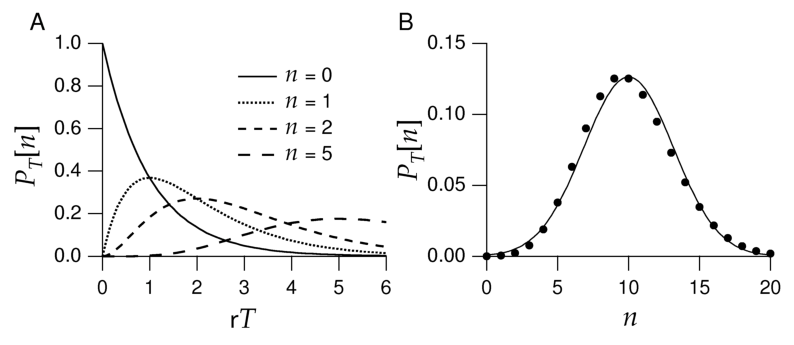
\includegraphics[height=5cm]{Poisson_graph.pdf}
    \caption{(Left) The probability that a homogeneous Poisson process generates $n$
spikes in a period $T$ plotted for $n = 0, 1, 2,$ and $5$ generalised as function of $\rho T$ to apply for any rate; (Right) The probability of $n$ spikes occurring for $\rho T= 10$ (dots) compared with a Gaussian distribution with mean and variance equal to $10$ (line). The figure is from \cite{Dyan-Abbott}.}
\end{figure}

\noindent
Figure 5 on the left shows this plotted for different values of $n$ as a function of $\rho T$ in order to apply for any value of the constant rate. The larger the number of spikes $n$ is the longer $T$ needs to grow in order for it to reach its maximum, i.e. The longer $T$ is the more likely it becomes to have more spikes occurring. On the right the probability mass function over possible numbers of spikes in is plotted showing that it matches a normal distribution around the expected fire rate.\\

\noindent
Now a simple procedure for generating spike trains from a Poisson
distribution can be designed using the estimated probability of firing
a spike within an interval of length $\delta t$ is $\rho\delta t$. As
the program progresses through time steps a random number between zero
and one is generated every time. If the probability of a spike is
higher than that number the time is recorded and added to the spike
train. The pseudocode for this is given below. This approach can be
used even if the fire rate $r(t)$ is not estimated by a constant but
depends on time, as long as it varies slowly with respect to the time
bin $\delta t$.\\

\begin{algorithm}[H]
  \KwIn{time period $T$, step length $\delta t$, expected firing rate $\rho$}
  \KwOut{spike train $\mathbf{u}$, spike count $c$}
  $\mathbf{u} \leftarrow [$ $]$\\
  \For {$i\leftarrow 1$ \KwTo $T/\delta t$}{
    $x_{rand} \leftarrow rand(0,1)$\\
    \If {$\rho \delta t > x_{rand}$}{
    	$\mathbf{u} \leftarrow \mathbf{u} \cup [i\delta t]$\\
        $c \leftarrow c + 1$\\
    }
  }
  \KwRet $\mathbf{u}, c$\\
  \vspace{11pt} \caption{Generating a Poisson neuron}
\end{algorithm}
\vspace{11pt}

\noindent
This concludes the introductory part. We now have all the necessary
components to build a model experiment for testing the
formula. The next chapter describes the experimental conditions simulated in
software to generate spike-train data for the model estimator. This is followed
by a documentation of the Python implementation of a simulation environment 
consisting of a spiking neural network, two spike-train metric measurements,
the mutual information estimator and the experimental procedures. This produces fictive 
data using a deterministic neural model that captures only the essential principle
of the real biophysical process. However, the level of abstraction is sufficient to
guarantee statistical relationships between spike train data analogous to the ones
expected to be seen in a real situation. The results form the conveyed trials are
then discussed and analysed in chapter four. 

%might need to add in a word for comparing with Bialek if added later on



\newpage
\section{Testing the model}
\subsection{Idea}

\noindent
Information theory establishes a relationship between the informativeness and
the probability distribution of the outcomes of random variables. It extends our
understanding about the meaning of structure in signals by enabling us
to measure how useful a piece of information is based on how likely we are to 
observe it. The notion of a \textit{random variable} itself, which in spite of its 
misleading name serves as a universal mathematical model of real processes, is 
better understood by extending the methods of probability theory and statistics
with the ones of information theory. The main motivation for applying information
theoretic analysis to neuroscientific data is quantifying the relationship between
a stimulus and a response.\\

\noindent
The estimation problem left aside, we are interested in measuring the information 
carried by a spike train response about a given stimulus. The stimulus can be the
spiking of a pre-synaptic neuron or it can be represented by a discrete variable
of some kind. In particular, we would like to separate the randomness observed in
spike trains that is directly influenced by the randomness of a particular stimulus, 
from the one which is due to noise propagating through the network via other synapting
neurons. This is exactly what mutual information measures. As seen in equation
\ref{MI(X;Y)=H(X)-H(X|Y)}, mutual information can be thought of as the uncertainty
associated with one variable taking away what would be left of it if another variable
were known. To put it differently it estimates the amount of information content present
in a variable due to its relationship with another variable. This information
measurement has no dependency on the actual values the variable takes or any statistic
associated with them. It is rather a statistic of the coding length due to their
improbability and as such is a direct product of their probability distribution.\\ 

\noindent
In order to test an information estimator using just a computer we want to design a
computational model generating multiple random variables related in a predefined way. We 
would then make a hypothesis about the expression of this relationship in terms of
mutual information and make the respective measurements using the formula in question.
Combining the framework of computational neuroscience with the spike-train metric
approach we can investigate the performance of the metric-space model for mutual
information and check if the results match our hypothesis. The kind of data which is
collected from electrophysological experiments with neurons can be mimicked by
simulating some neurons using the integrate-and-fire model while feeding them
randomly generated pre-synaptic spiking with firing rates coming from a Poisson
distribution. As outlined above the kind of spike trains generated using the Poisson
model imitate neural activity resulting from the rich connectivity observed in many 
real neural networks.\\

\noindent
To produce the desired statistical relationship we would like to set up a network 
comprised of both types of artificial neurons and simulate its voltage dynamics over 
multiple trials under the same experimental conditions. In this way we can generate
enough data to apply the metric-space method for information estimation which relies on
nearest neighbour statistics between spike train sample points. By then varying certain
experimental parameters we can observe the resulting tendencies in the mutual
information variation and compare then to our expectations.



\subsection{Experimental network set-up}
\begin{figure}[H]
	\centering
	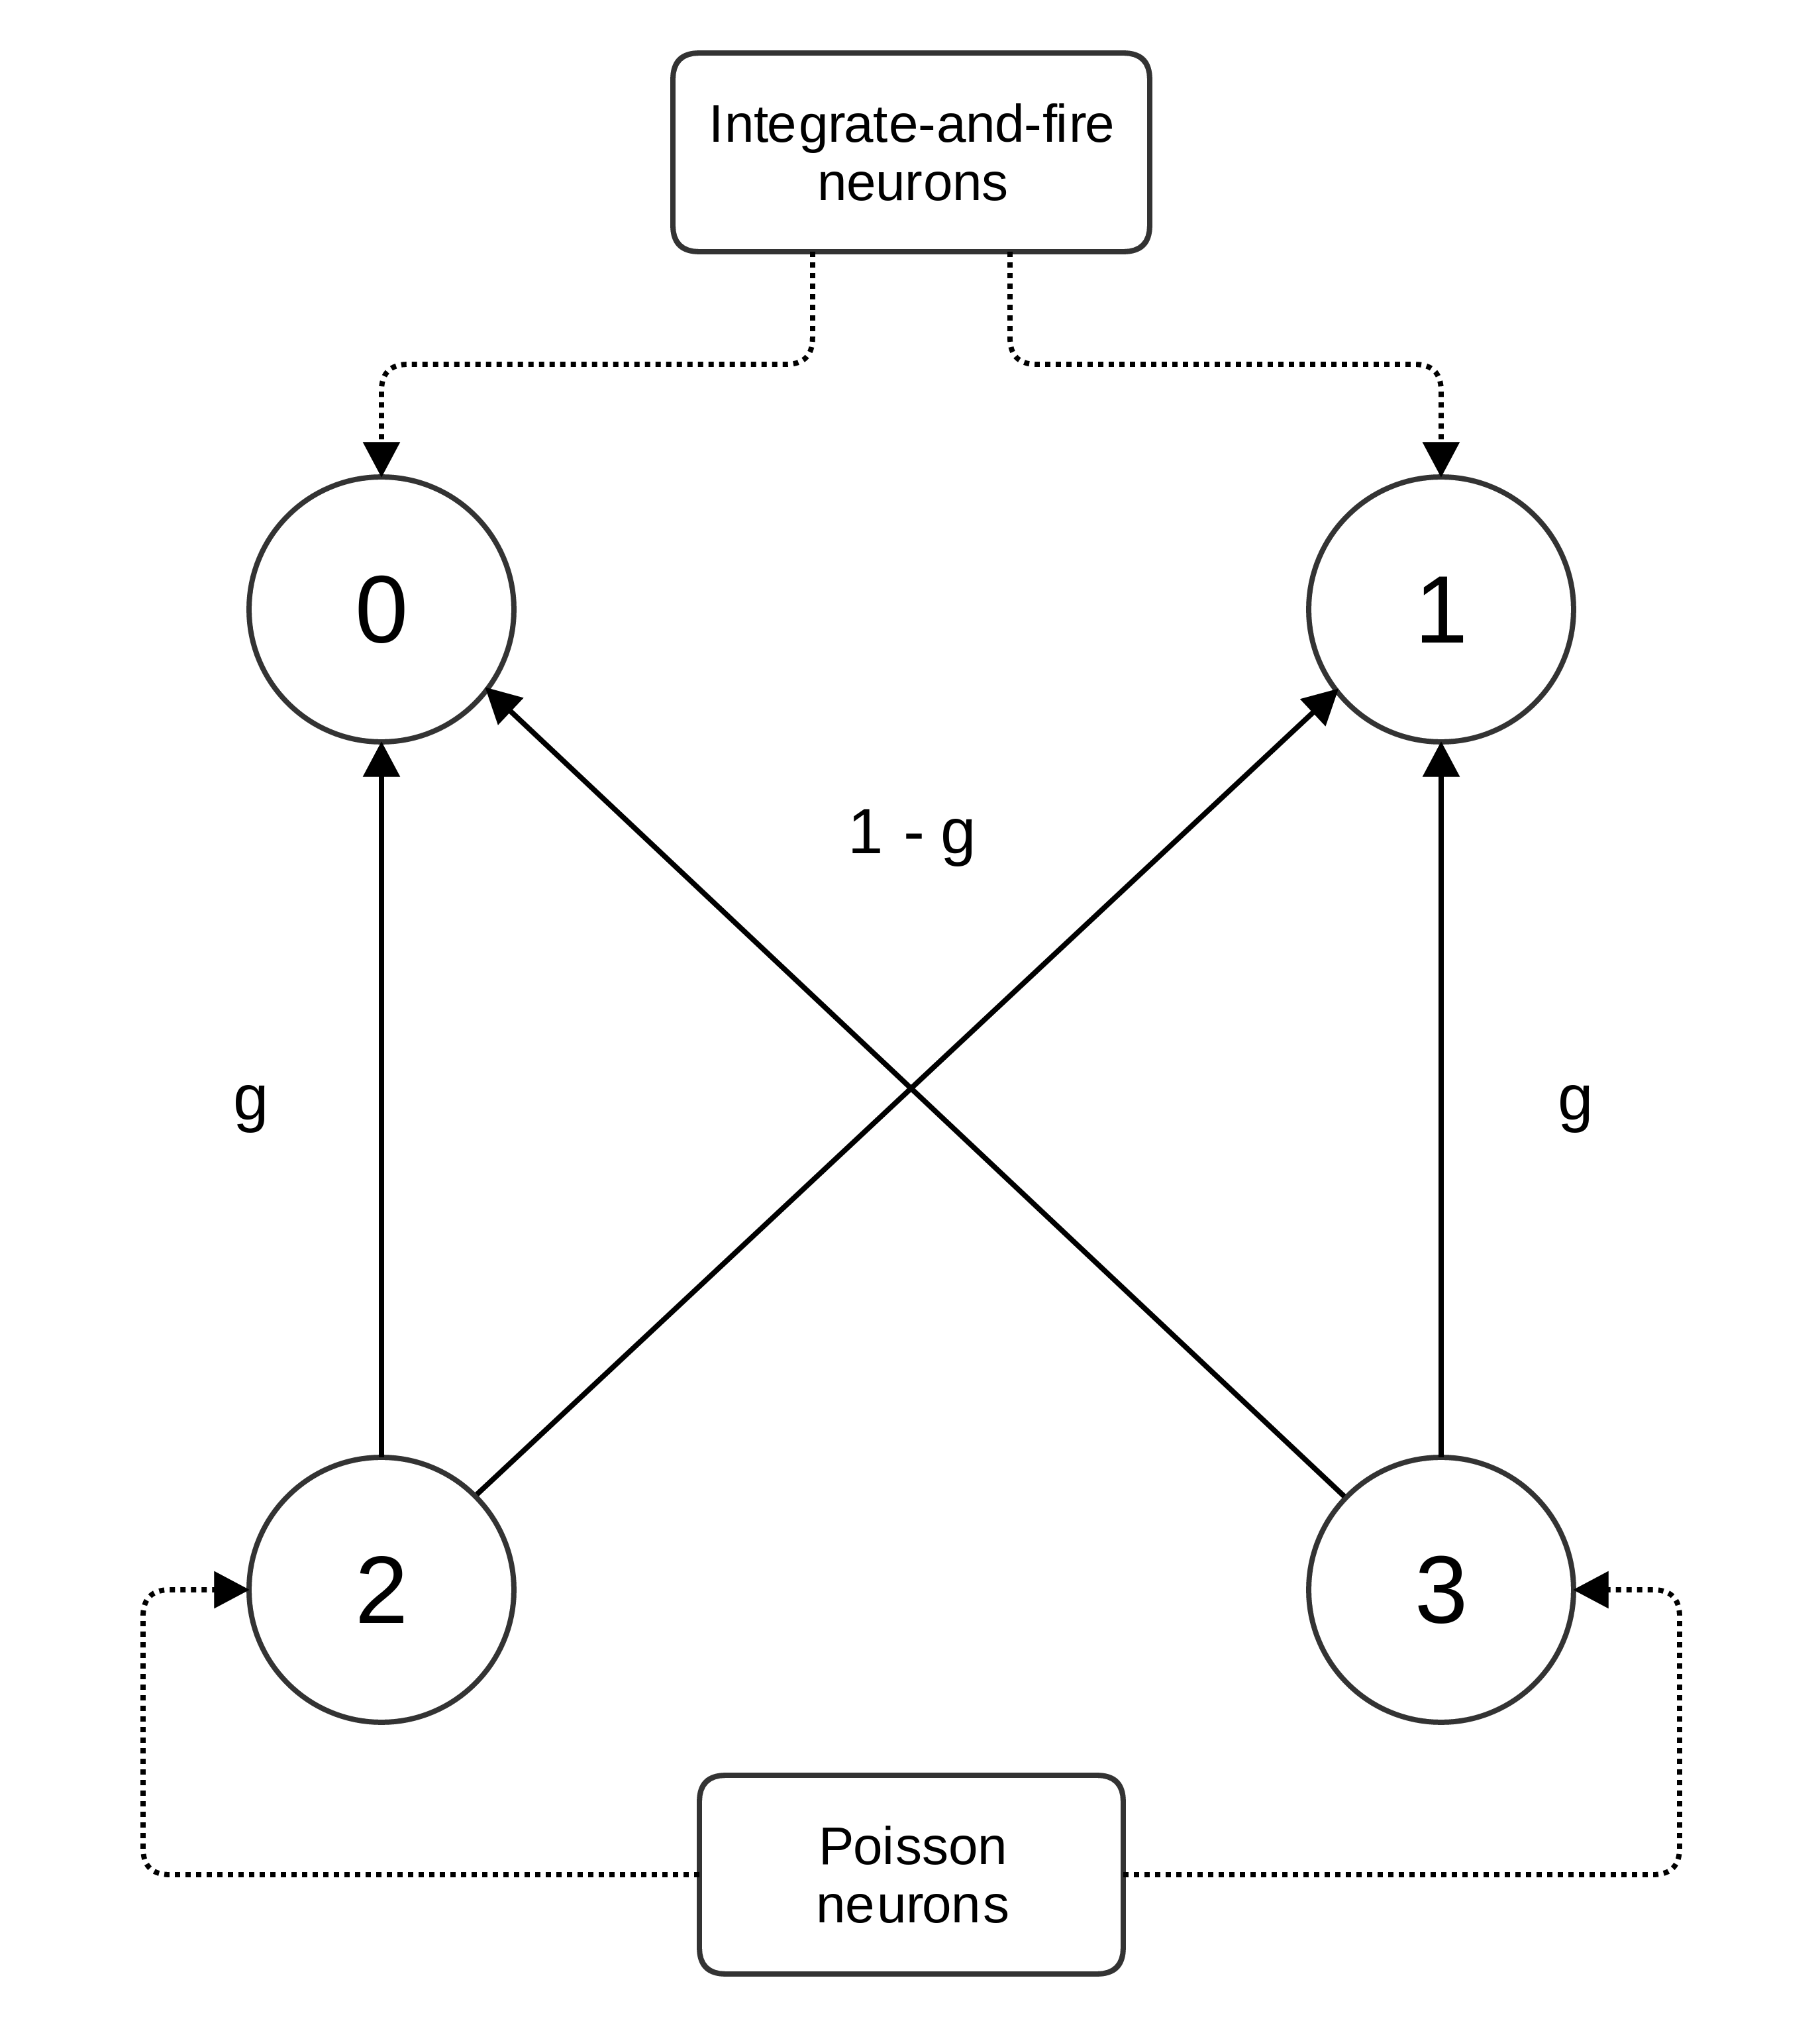
\includegraphics[height=12cm]{exp_net_23.png}
    \caption{}
\end{figure}

\subsection{Experiment 1: Mutual information vs. synapse strength}

\subsection{Experiment 2: Mutual information vs. stimulus delay}

\subsection{Reverse engineering the network}
\begin{figure}[H]
	\centering
	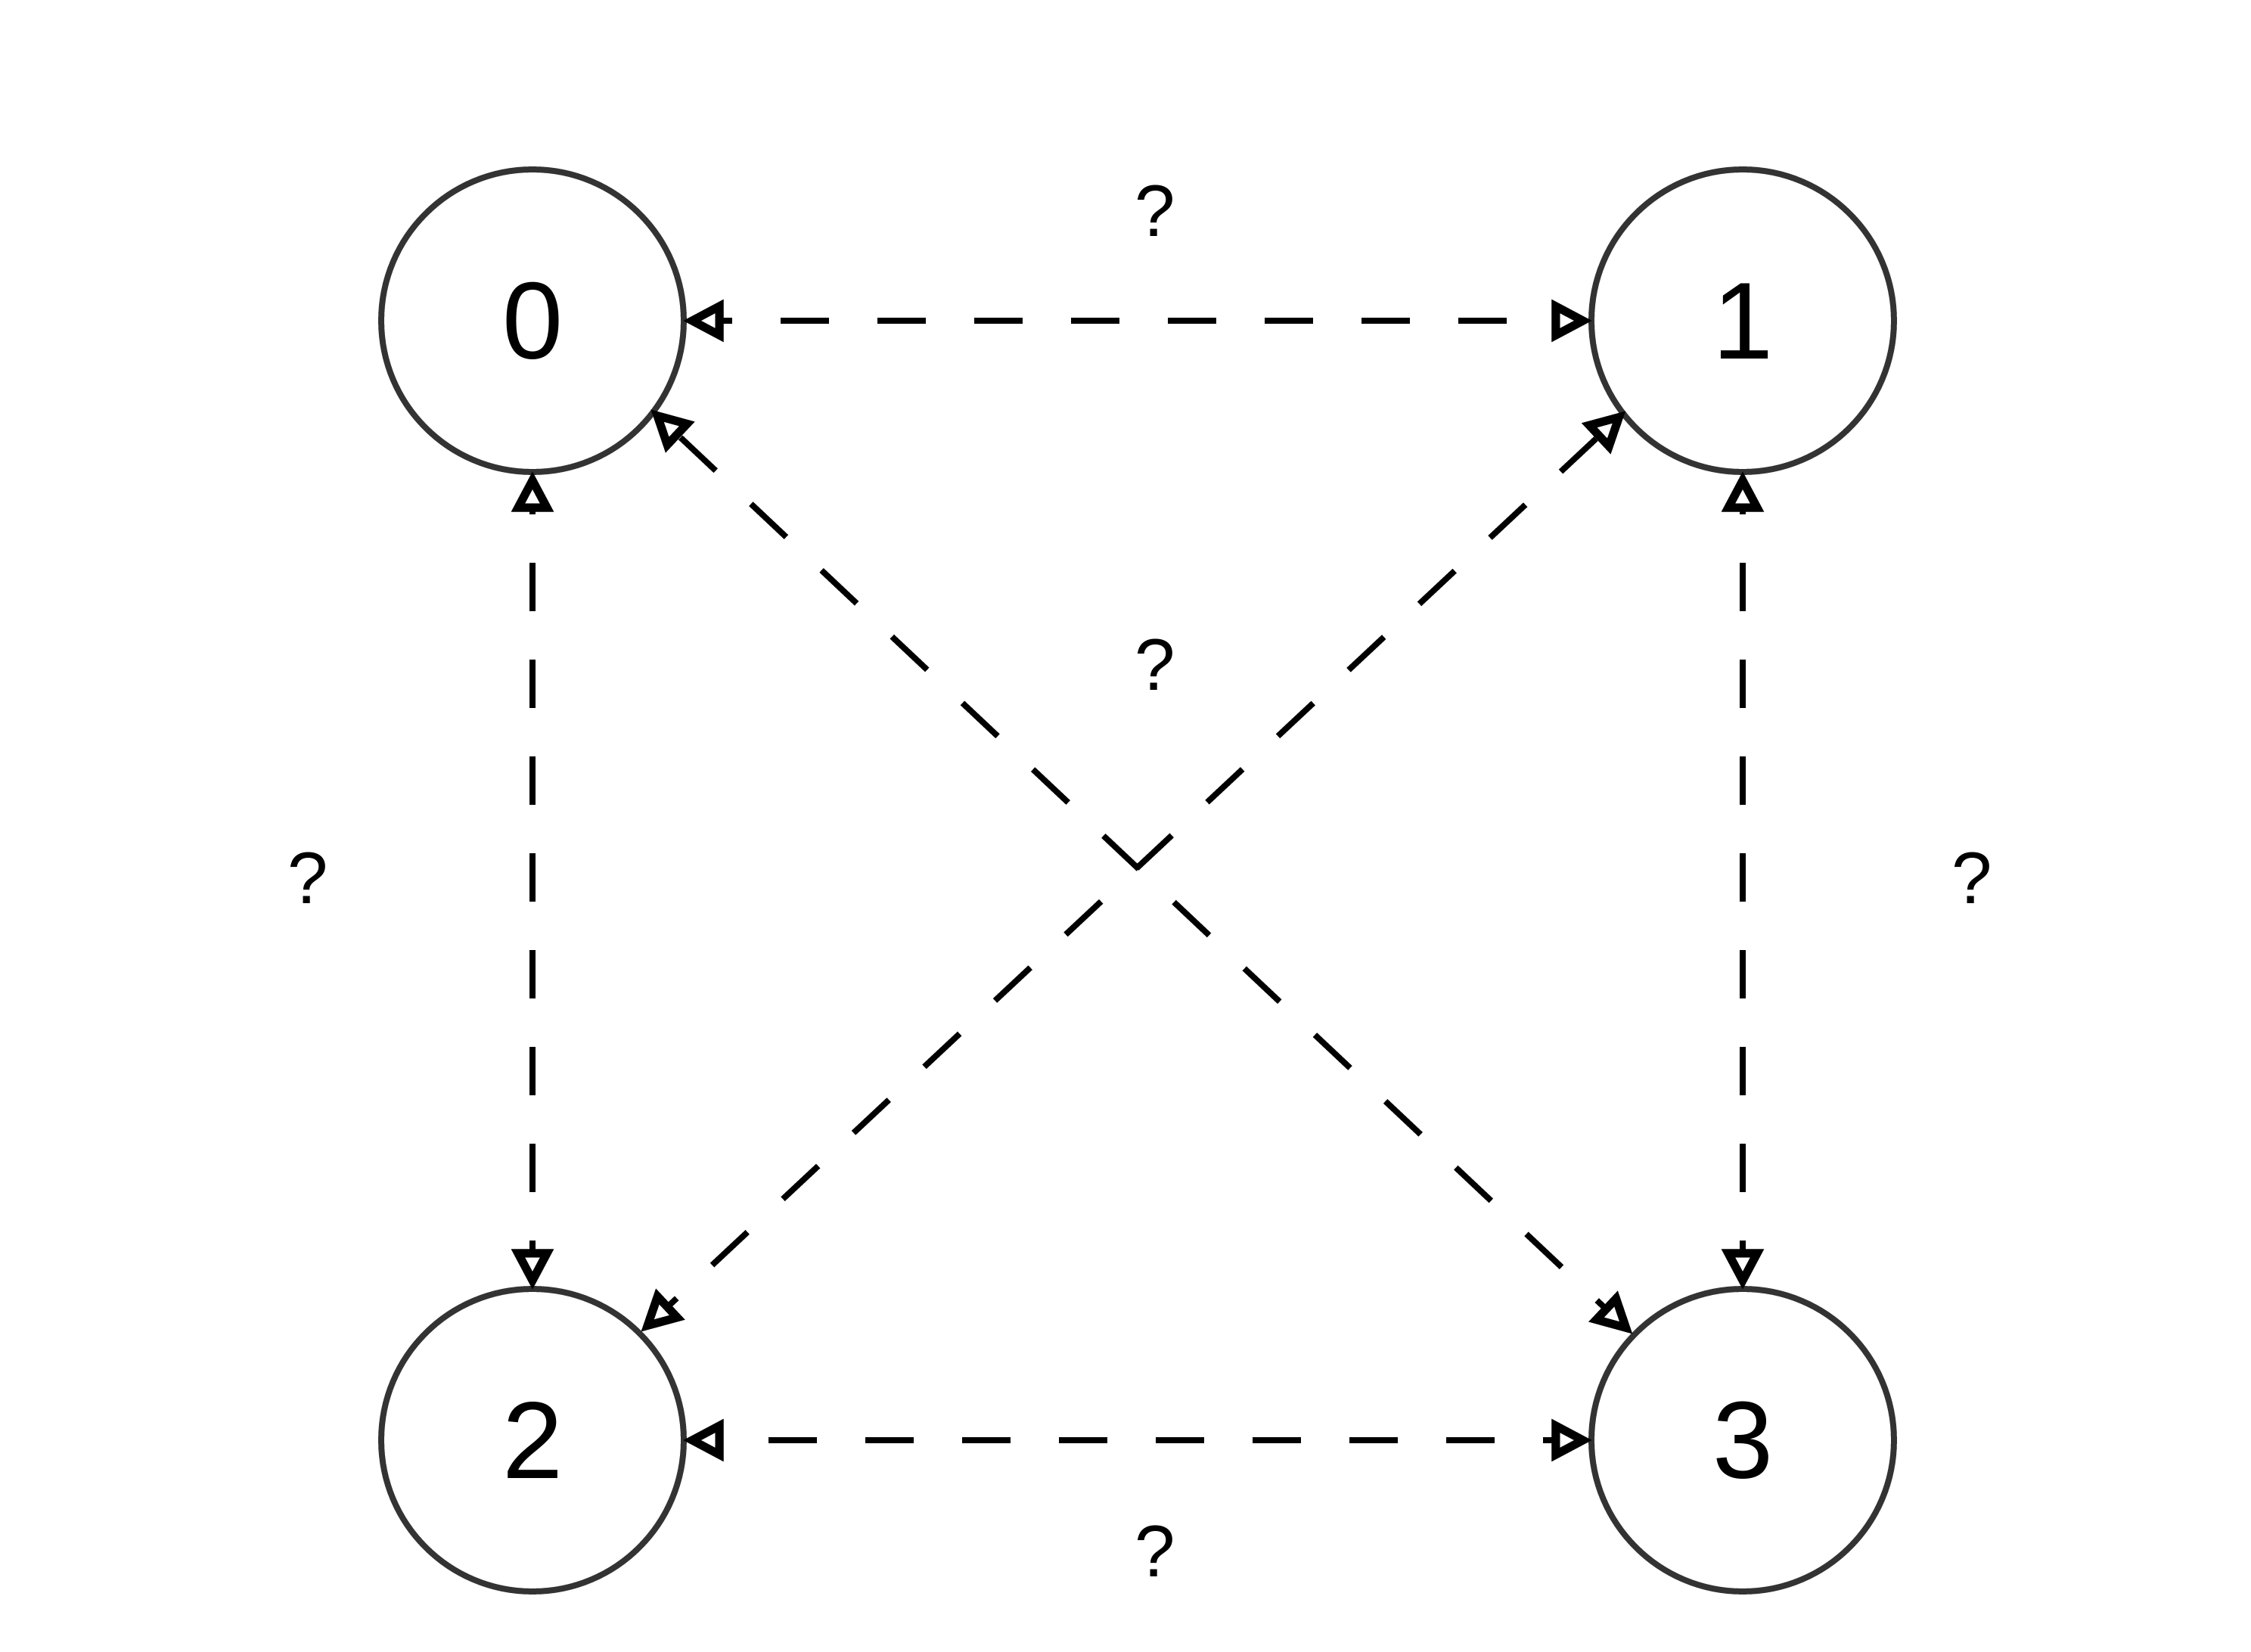
\includegraphics[height=9cm]{exp_net_23_naked.png}
    \caption{}
\end{figure}




\newpage
\section{Implementation}
\subsection{Integrate and fire neurons}
\begin{figure}[H]
	\centering
	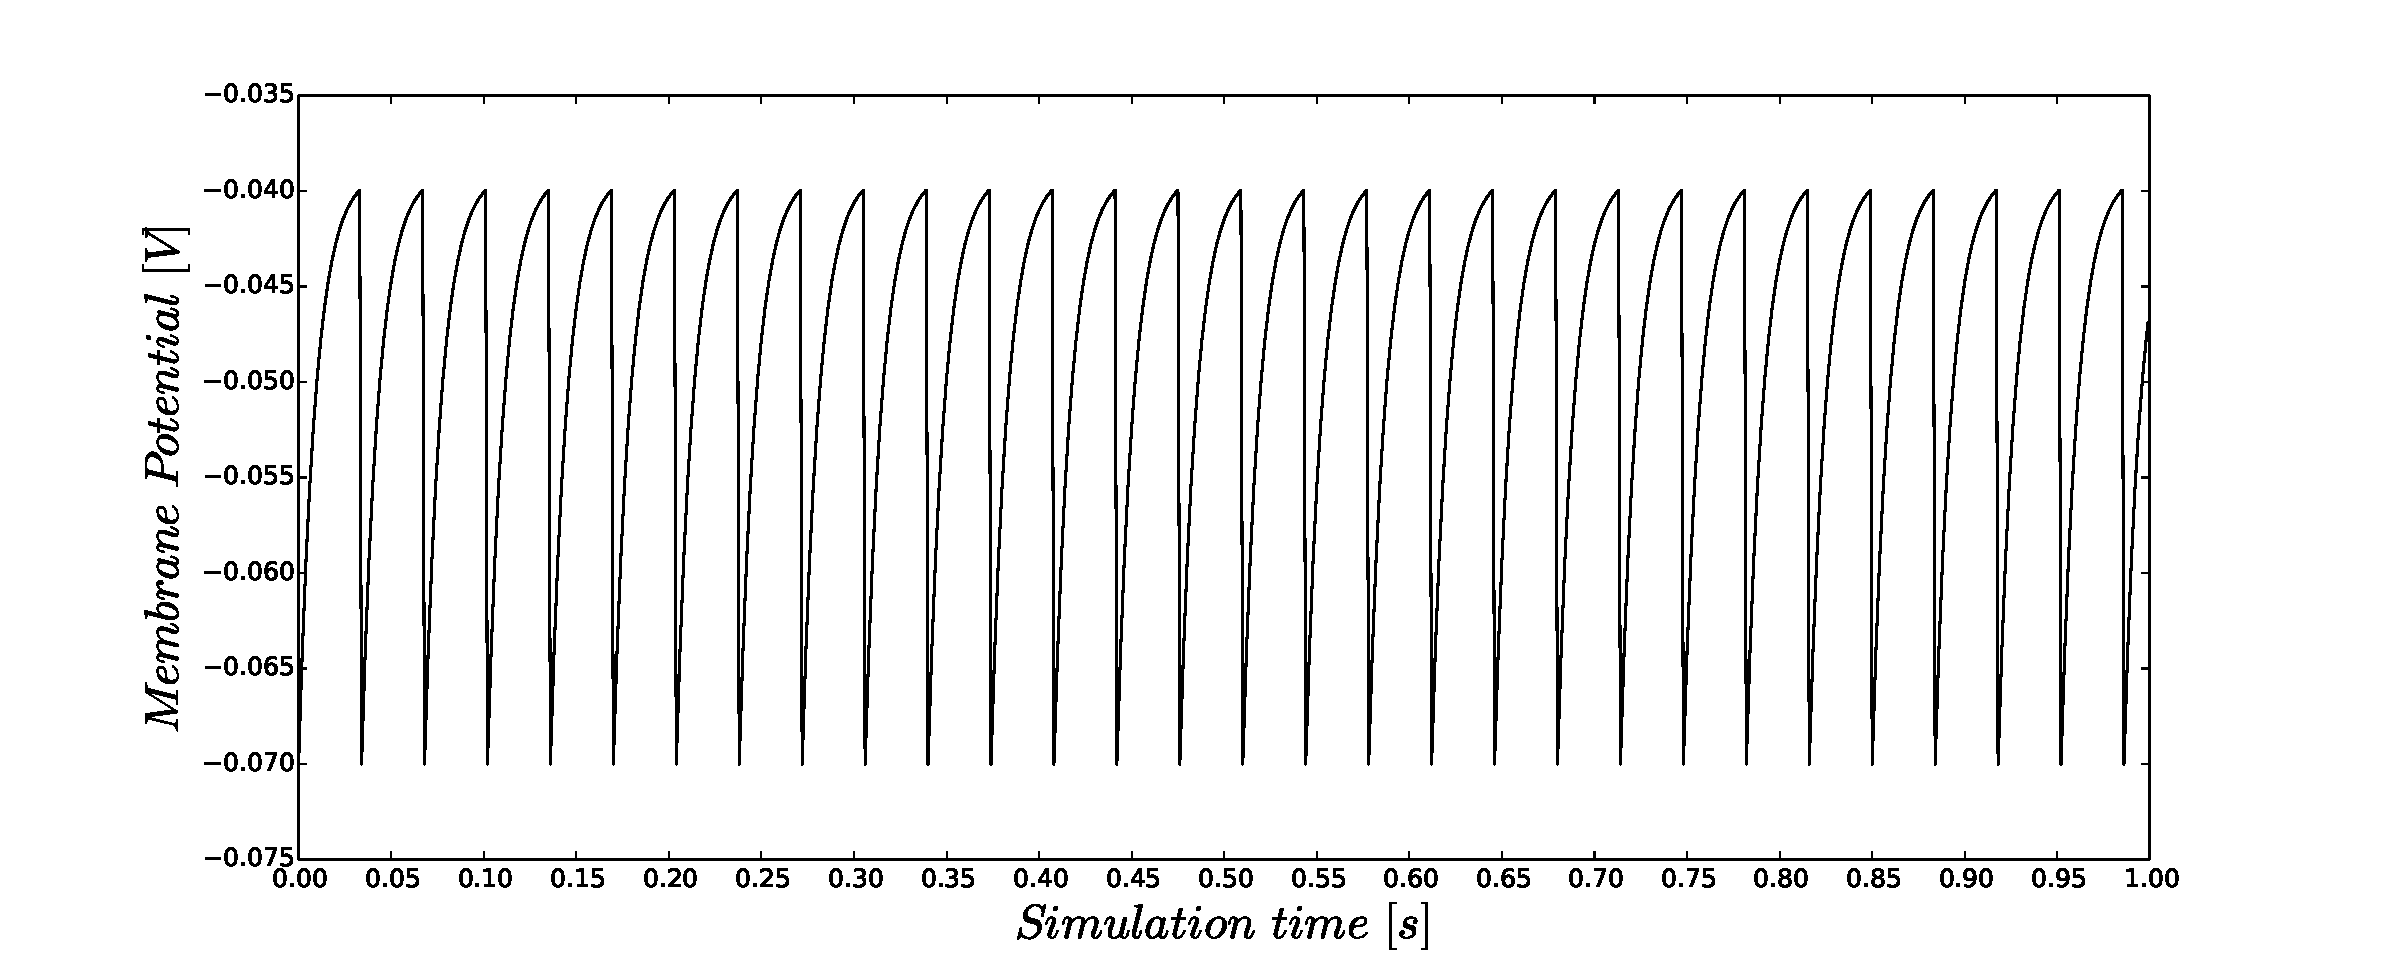
\includegraphics[width=\textwidth]{LIF_spiking_1s.pdf}
    \caption{}
\end{figure}

\begin{figure}[H]
	\centering
	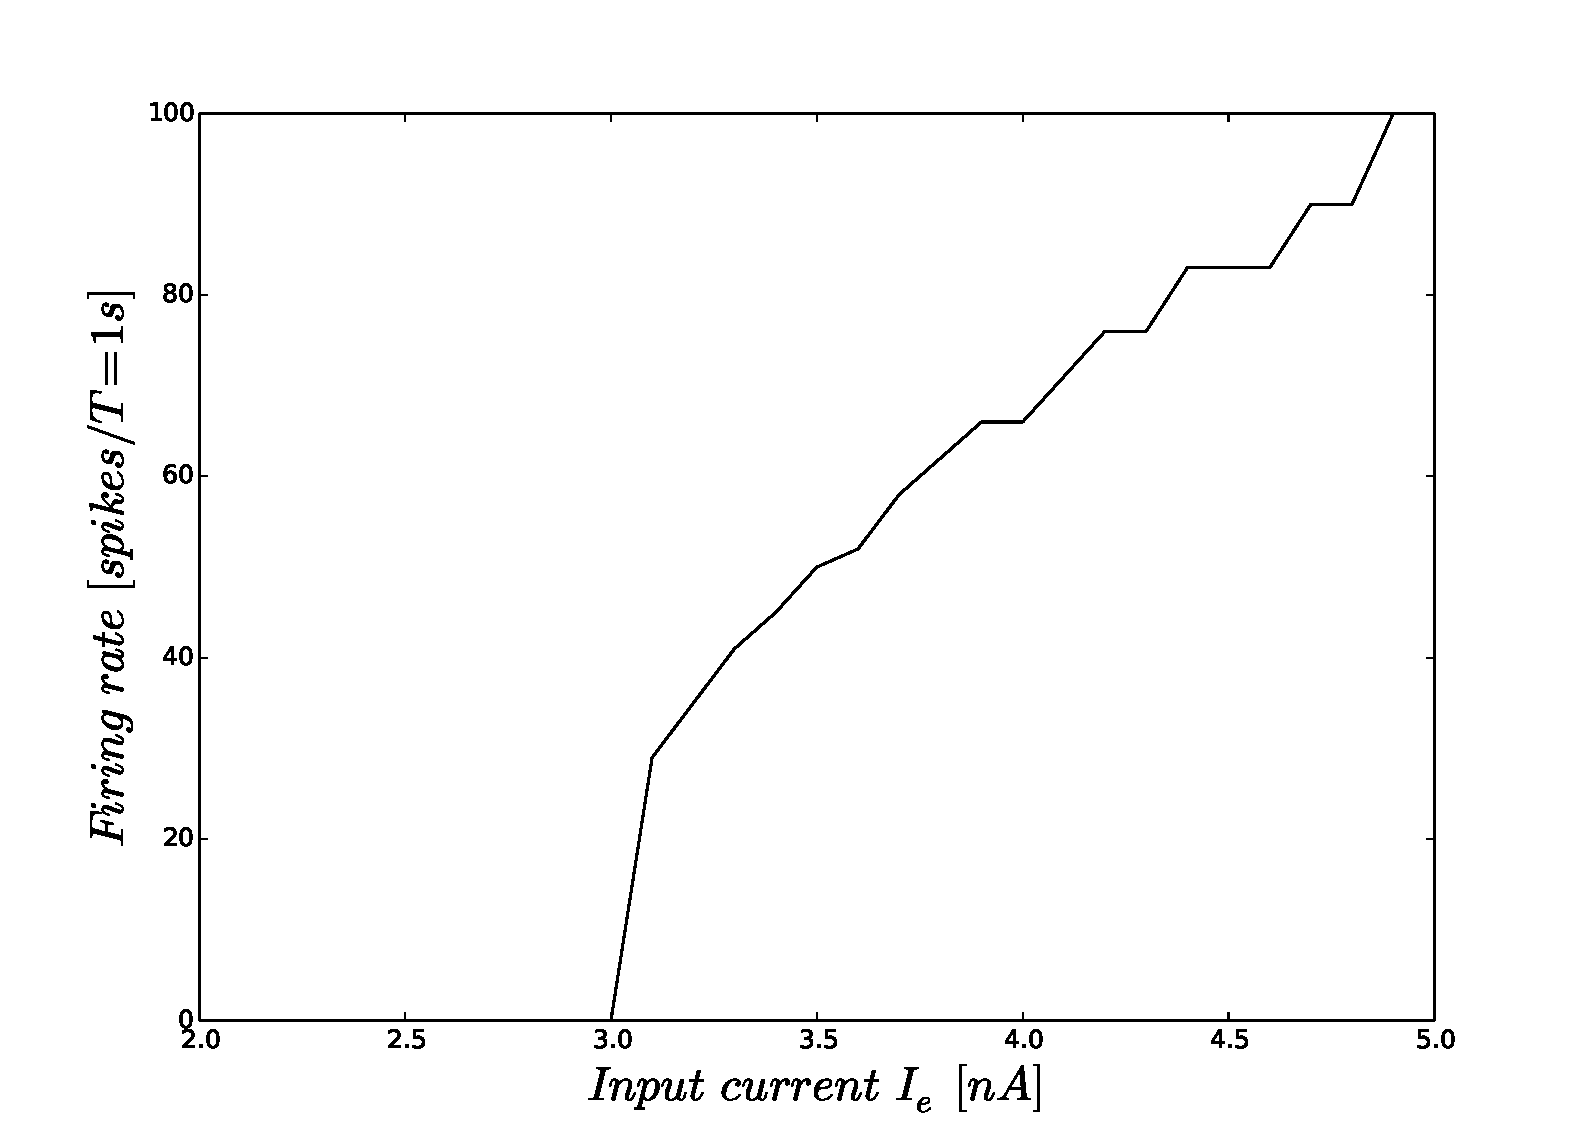
\includegraphics[height=9cm]{LIF_spikint_rate_vs_incurrent.pdf}
    \caption{}
\end{figure}

\subsection{Poisson neurons}

\subsection{Network simulation}

\subsubsection*{Two coupled neurons}
\begin{figure}[H]
	\centering
	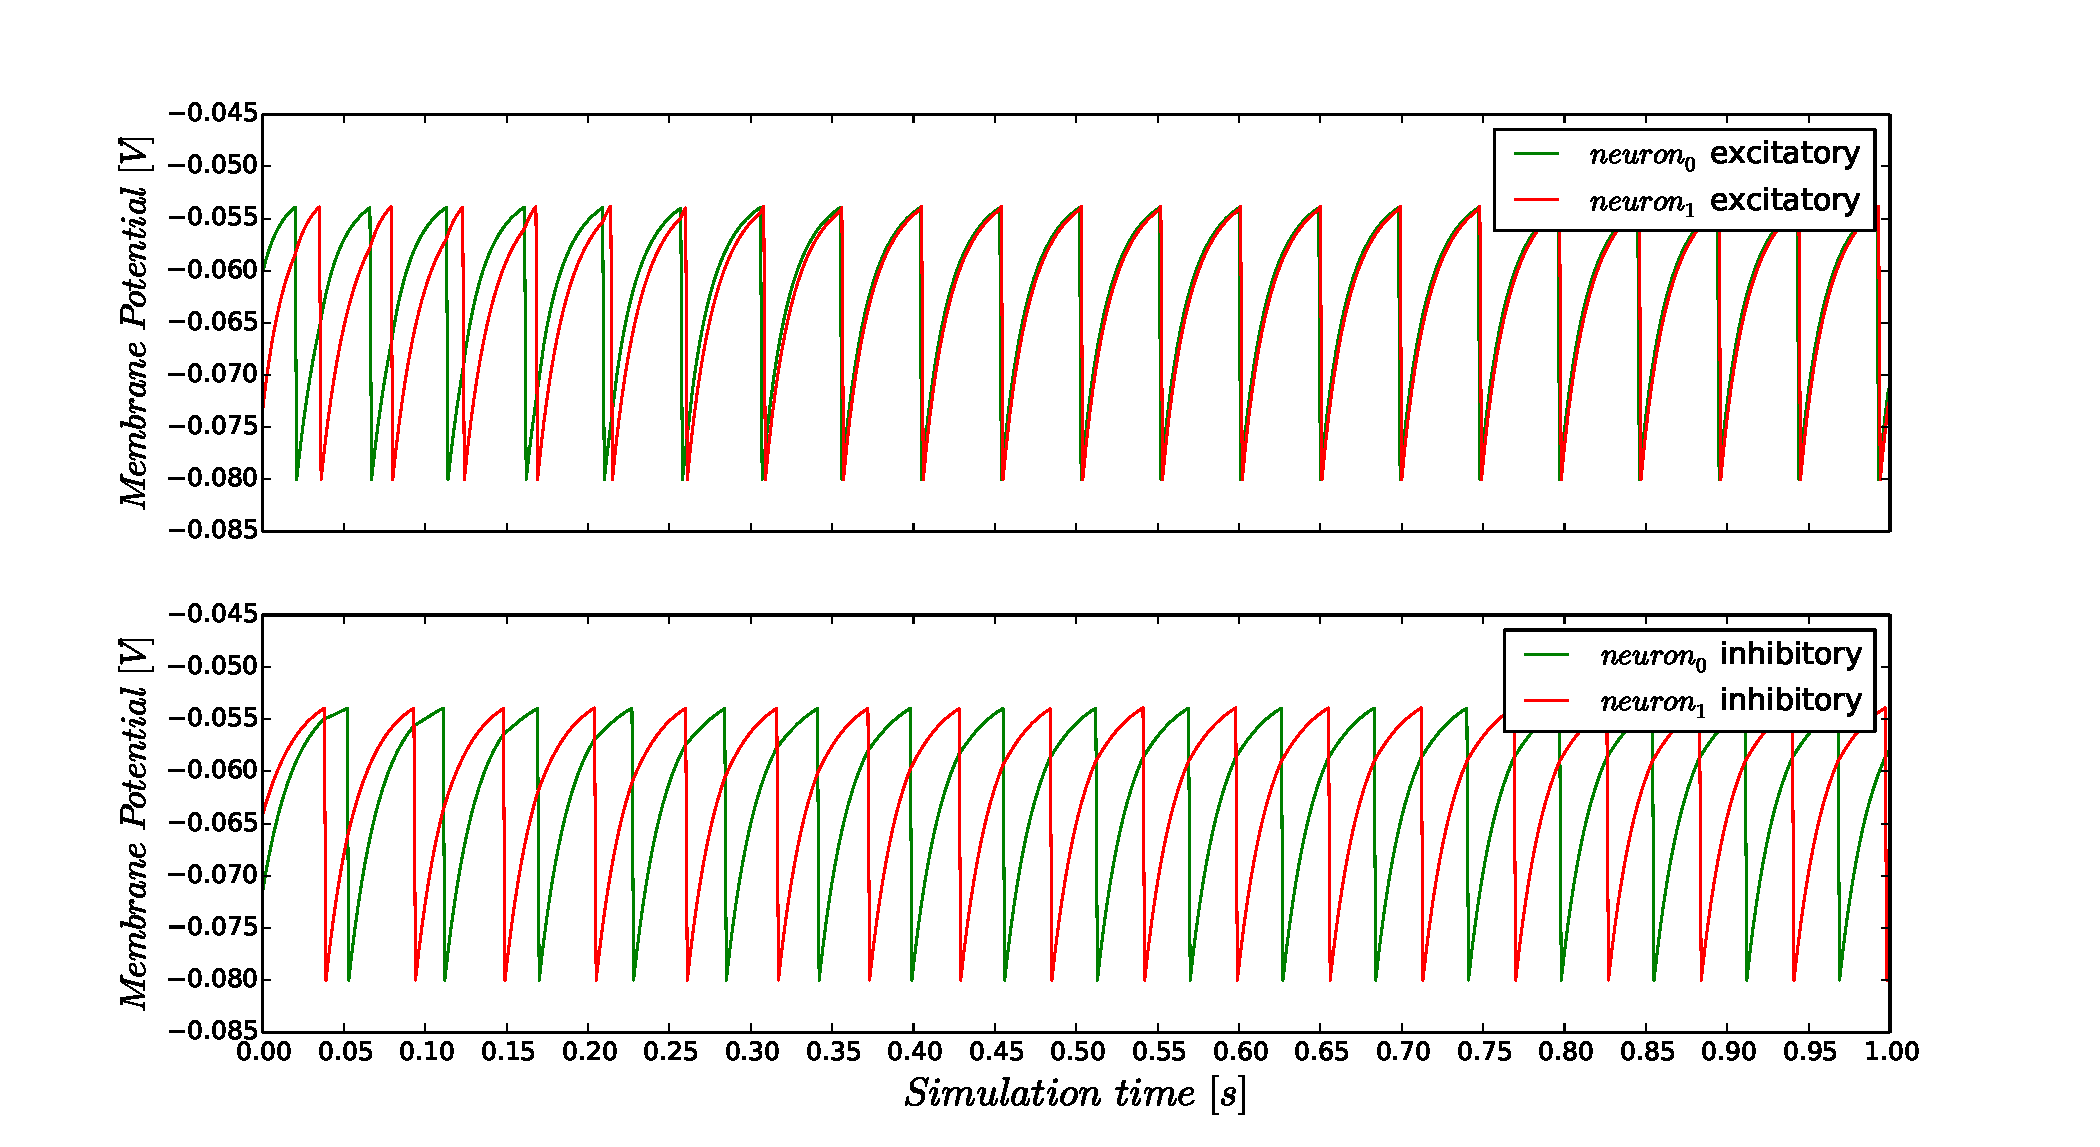
\includegraphics[width=\textwidth]{LIF_spiking_1x1_1s.pdf}
    \caption{}
\end{figure}

\subsubsection*{Propagation network}
\begin{figure}[H]
	\centering
	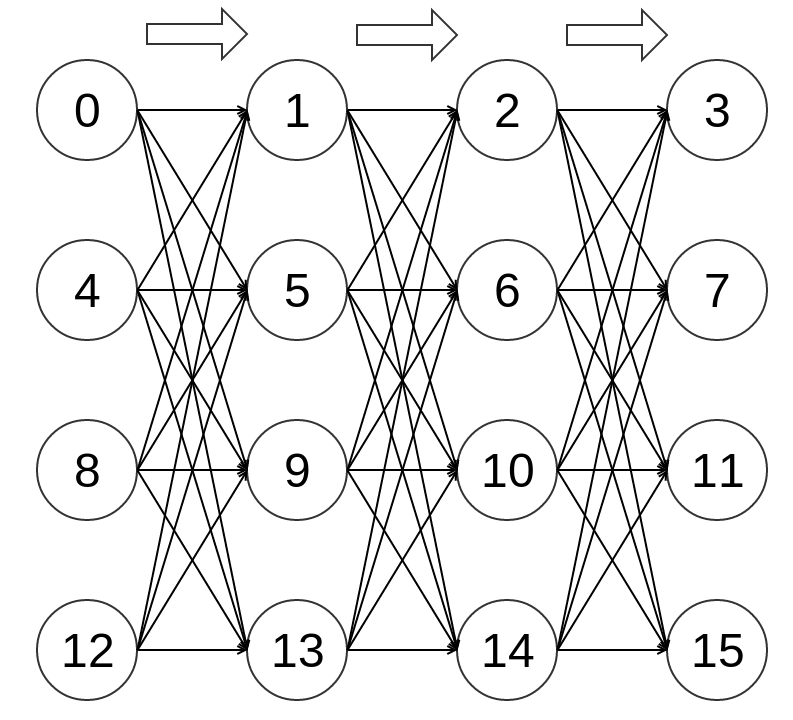
\includegraphics[height=7cm]{4x4_layered_full_conn.png}
    \caption{}
\end{figure}


\begin{figure}[H]
	\centering
	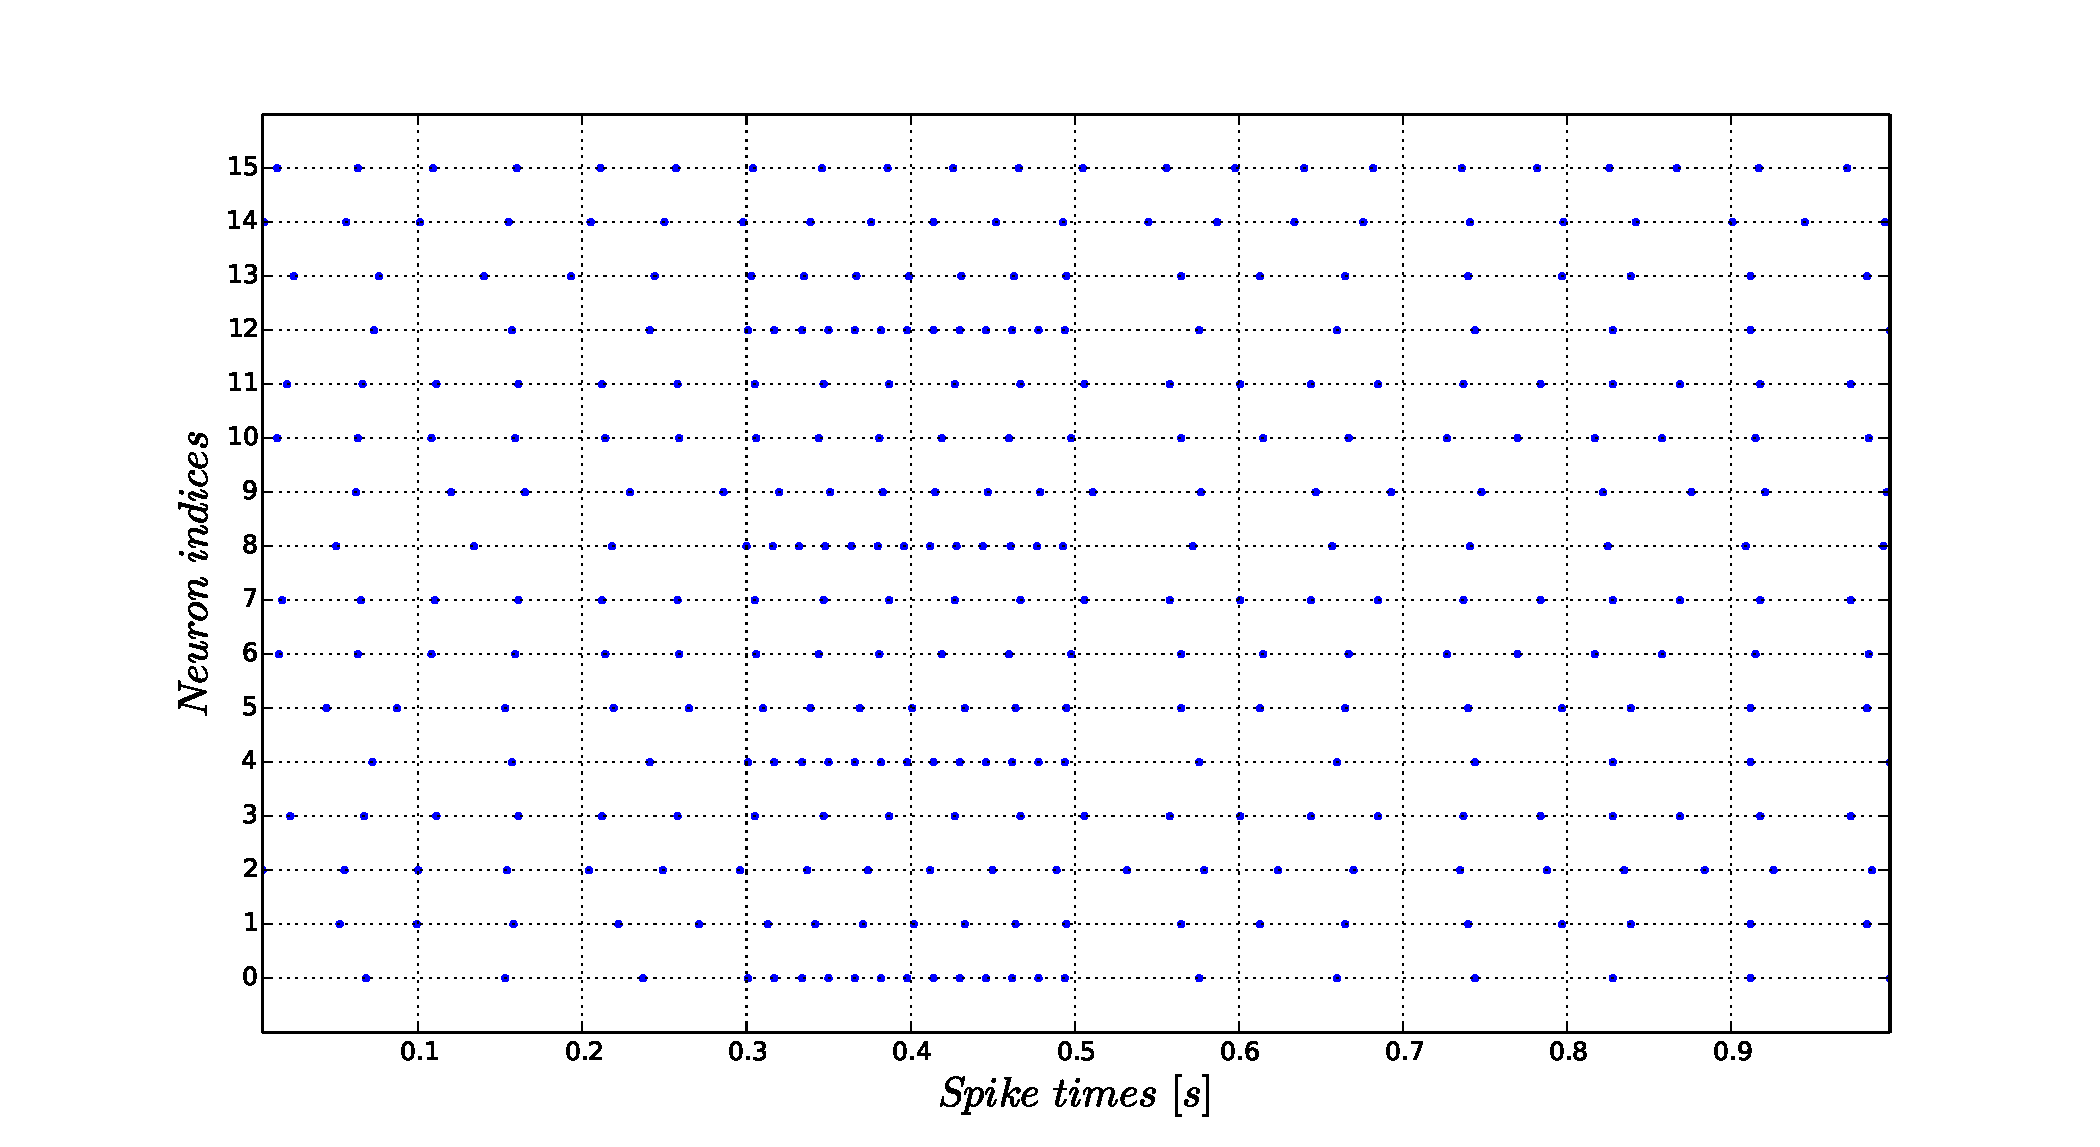
\includegraphics[width=\textwidth]{raster_4x4_layered_full_crop.pdf}
    \caption{}
\end{figure}

\subsection{Computing distances}

\subsection{Estimating mutual information}




\newpage
\section{Results}
\subsection{Experiment 1}
\begin{figure}[H]
	\centering
	\includegraphics[width=\textwidth]{MI_2_0_50x48_12x12_poisson_rates_in_u_10-50__VP_120dpi.pdf}
    \caption{}
\end{figure}


\begin{figure}[H]
	\centering
	\includegraphics[width=\textwidth]{MI_2_1_50x48_12x12_poisson_rates_in_u_10-50__VP_120dpi.pdf}
    \caption{}
\end{figure}


\subsection{Experiment 2}

\begin{figure}[H]
	\centering
	\includegraphics[width=\textwidth]{DELAY_MI_2_0_120x300_40x40_poisson_rates_in_U_10-20__vR.pdf}
    \caption{}
\end{figure}


\begin{figure}[H]
	\centering
	\includegraphics[width=\textwidth]{DELAY_MI_2_0_37x23x48_12x12_poisson_rates_in_U_10-20__vR_with_std_devs_120dpi.pdf}
    \caption{}
\end{figure}


\subsection{Connectivity inference}

\begin{figure}[H]
	\centering
	\includegraphics[width=\textwidth]{MI_MIXED_PAIRWISE_50x48_12x12_pRates_U_10-50__VP_120dpi.pdf}
    \caption{}
\end{figure}

\begin{figure}[H]
	\centering
	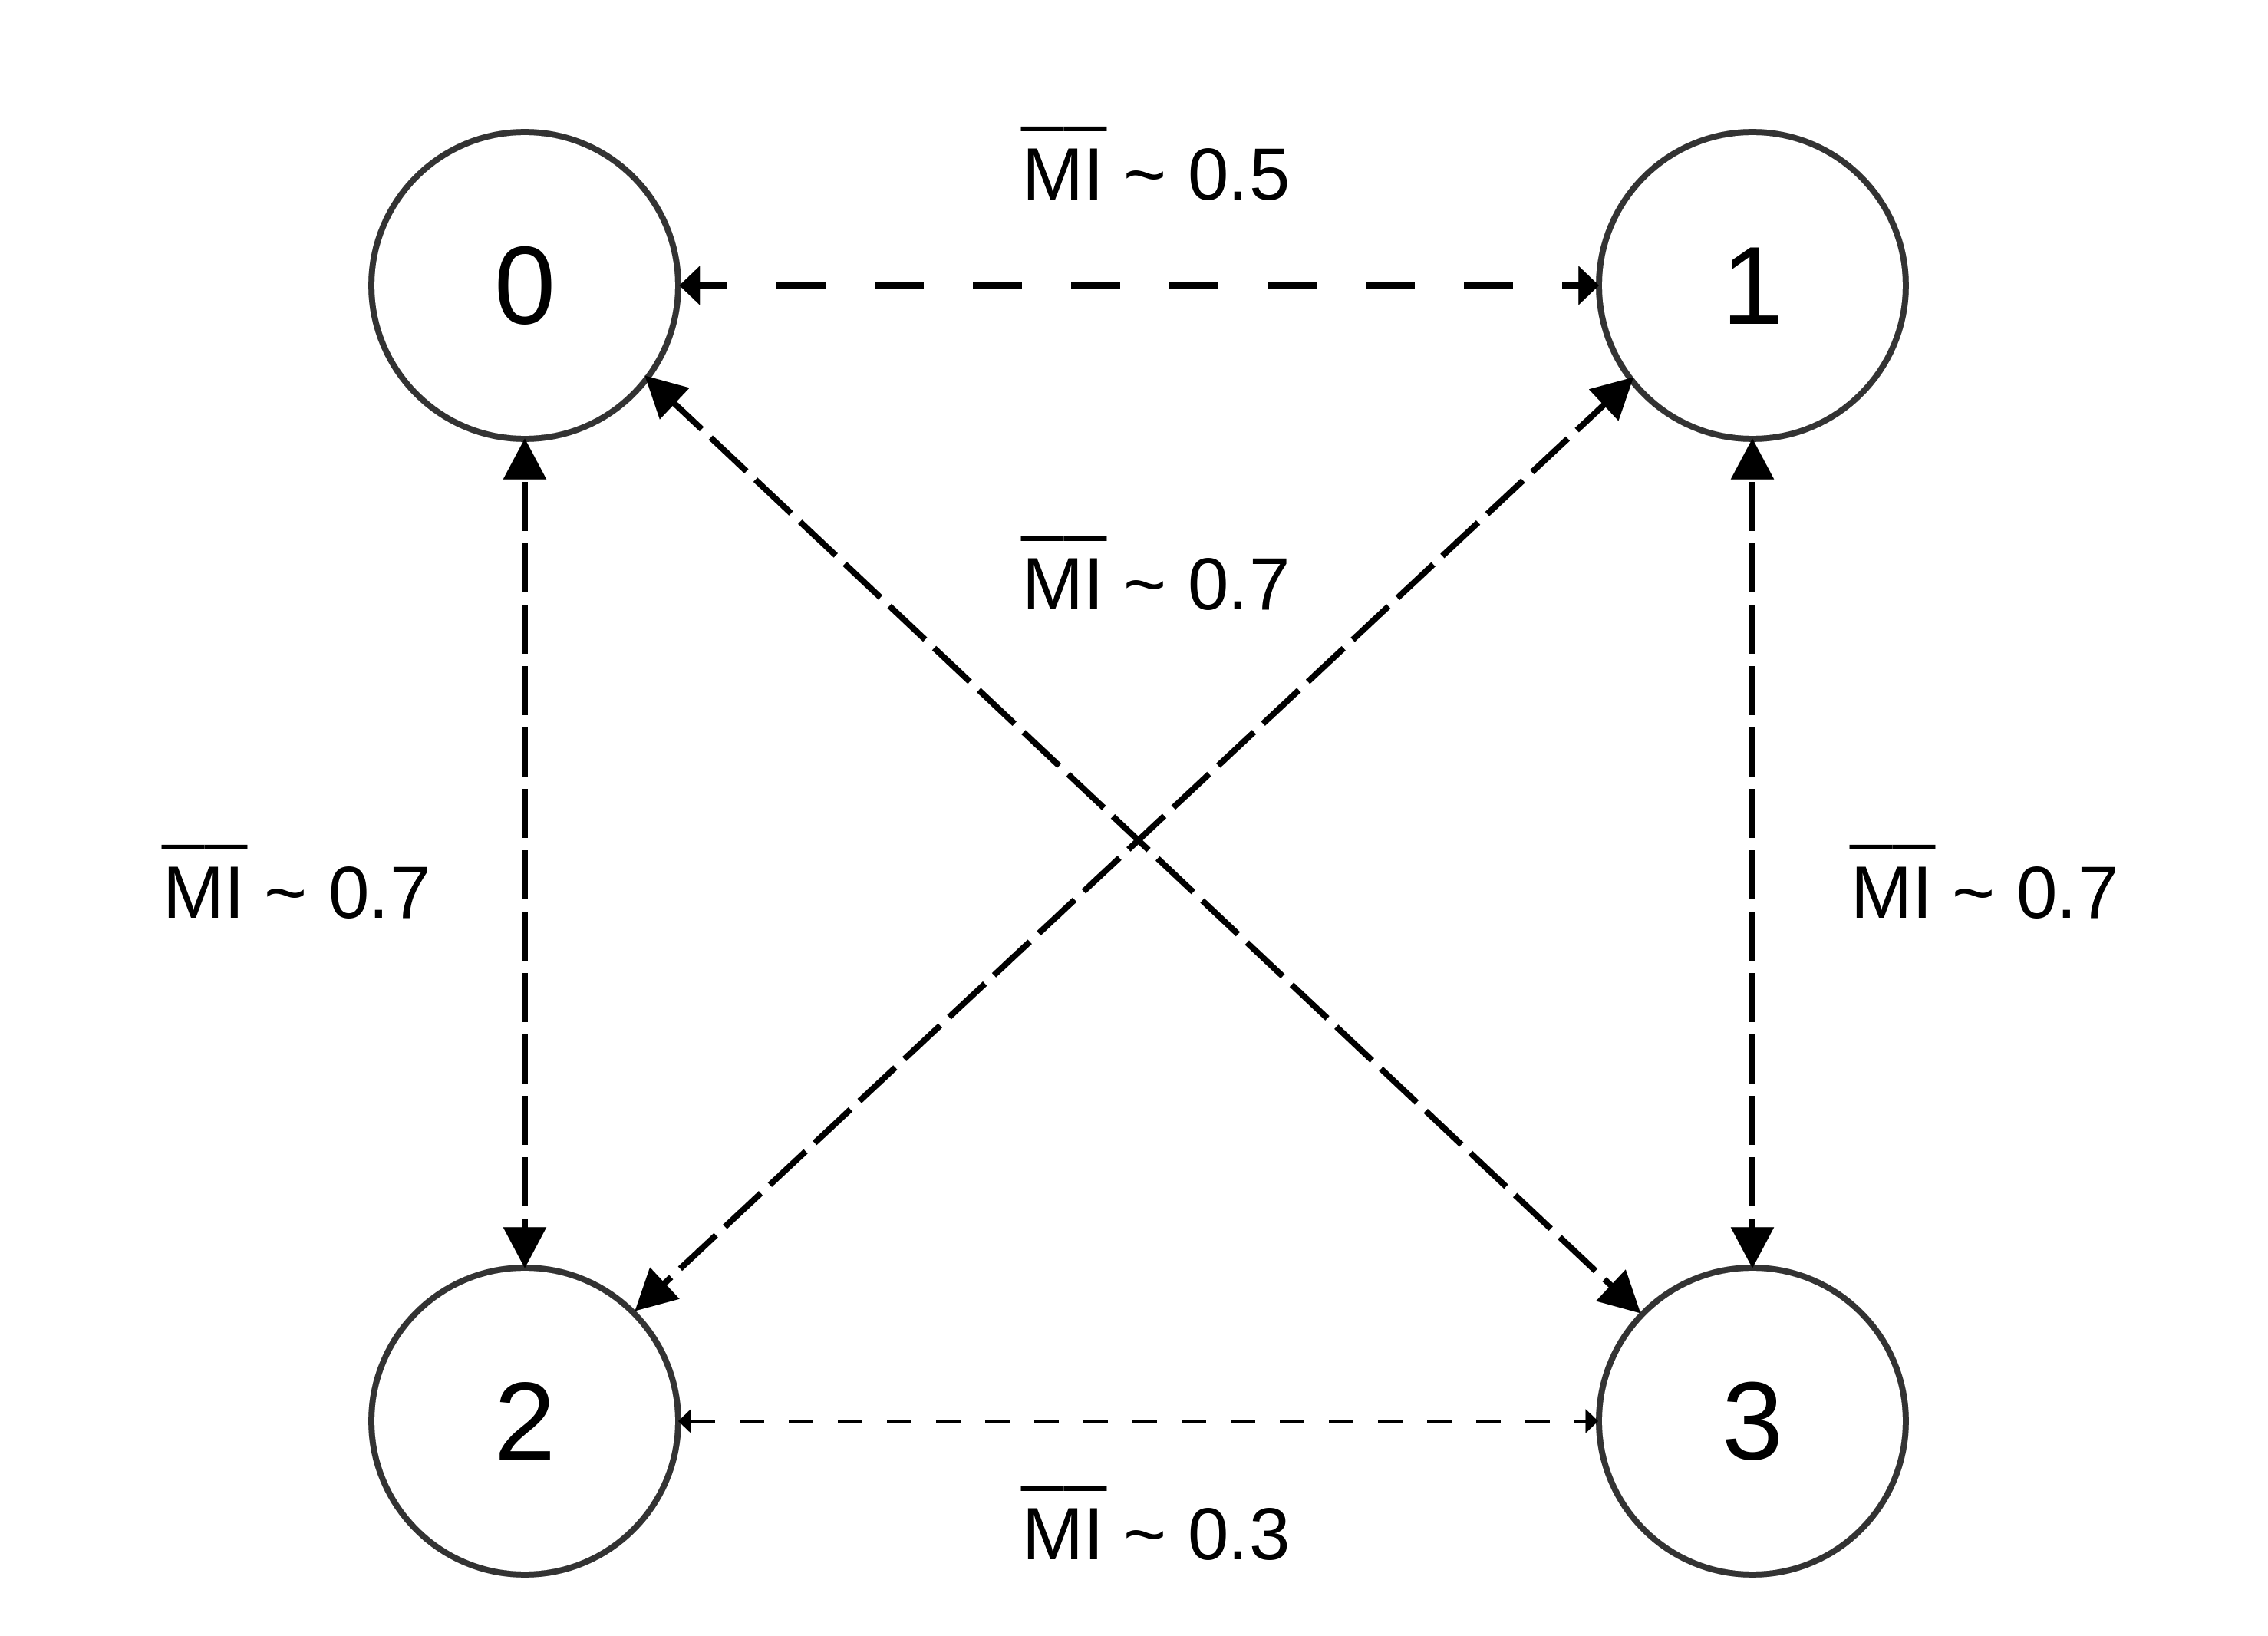
\includegraphics[height=9cm]{exp_net_23_full_naked.png}
    \caption{}
\end{figure}


\newpage
\addcontentsline{toc}{section}{Conclusions}
\section*{Conclusions}




\newpage
\addcontentsline{toc}{section}{References}
\small{
\begin{thebibliography}{} 
	 \bibitem{Lapique}{Lapicque L. (1907). Recherches quantitatives sur l’excitation lectrique des nerfs traite comme une polarisation. \textit{J. Physiol. Pathol. Gen}, 9:620–635.}
     
	\bibitem{Shannon}{Shannon CE. (1948) A mathematical theory of communication. \emph{Bell Syst. Tech. J.}, 27: 379-423,623-656.}
    
    \bibitem{Hodgkin-Huxley}{Hodgkin AL and Huxley HF. (1952) Propagation of electrical signals along giant nerve fibres. \textit{Proceedings of the Royal Society of London. Series B, Biological Sciences}, 140:177-183.}
    
    \bibitem{Dobrushin}{Dobrushin RL. (1958) A simplified method for experimental estimate of the entropy of a stationary sequence \textit{Theory Prob. Appl. 3}, 462}
    
    \bibitem{Kozachenko-Leonenko}{Kozachenko LF, Leonenko NN. (1987) Sample estimate of the entropy of a random vector. \emph{Probl. Pereda. Inf.}, 23: 9–16.}
    
    \bibitem{Num.recepies.in.C}{Press WH, Teukolsky SA, Vetterling WT and Flannery BP. (1988) ``Numerical recipes in C". \textit{Cambridge University Press.}, p.710-714.}
    
     \bibitem{Victor-Purpura_1}{Victor JD and Purpura KP. (1996) Metric-space analysis of spike trains: theory, algorithms and application. \textit{Network: Computation in Neural Systems}, 8:127-164.}   
    
    \bibitem{Victor-Purpura_2}{Victor JD and Purpura KP. (1996) Nature and precision of temporal coding in visual cortex: a metric-space analysis. \textit{Journal of Neurophysiology}, 76:1310-1326}
    
    \bibitem{Victor-Reich}{Reich DS, Victor JD, Knight BW, Ozaki T, Kaplan E. (1997) Response variability and timing precision of neuronal spike trains in vivo. \textit{Journal Neurophysiology}, 77:2836-2841.}
    
    \bibitem{STRONG}{Strong SP, Koberle R, de Ruyter van Steveninck RR, Bialek W. (1998) Entropy and information in neural spike trains \textit{Phys. Rev. Lett. 80}, 197-200}
    
    \bibitem{Rubner.Earth-mover}{Rubner Y, Tomasi C, Guibas LJ. (2000) The earth mover's distance as a metric for image retrieval. \textit{International Journal of Computer Vision}, 40:99‐121.}
    
    \bibitem{Dyan-Abbott}{Dayan P and Abbott L. (2001) ``Theoretical Neuroscience" \textit{MIT Press}, Chapter 1.4.}
    
    \bibitem{van.Rossum}{van Rossum M. (2001) A novel spike distance. \textit{Neural Computation}, 12:751-763.}
    
    \bibitem{Victor.2002}{Victor JD. (2002) Binless strategies for estimation of information from neural data. \textit{Phys. Rev. E}, 66, 051903.} 

    \bibitem{Kraskov}{Kraskov A, St\"{o}gbauer H, Grassberger P. (2004) Estimating mutual information. \emph{Phys. Rev. E}, 69, 066138.}
    
    \bibitem{Thomas}{Cover TM, Thomas JA. (2006) ``Elements of information theory" -2nd ed. \emph{A Wiley-Interscience publication.}, p.13-57 ISBN-13 978-0-471-24195-9.}
    
    \bibitem{Houghton-Victor}{Houghton CJ, Victor JD. (2012) Measuring representational distances -- the spike-train metrics approach. \textit{``Visual population codes: toward a common multivariate framework for cell recording and functional imaging". (eds N Kriegeskorte, G Kreiman) Cambridge, MA: MIT Press}, p.391-416.}
    
    \bibitem{Houghton-Kreuz.12}{Houghton CJ and Kreuz T. (2012) On the efficient calculation of van Rossum distances. \textit{Network computation in neural systems}, 23(1-2):48-58.}
    
    \bibitem{Tobin-Houghton}{Tobin RJ, Houghton CJ. (2013) A kernel-based calculation of spike train information. \textit{Entropy 15}, 4540–4552.}
    
    \bibitem{Kinney-Atwal}{Kinney JB and Atwal GS. (2014) Equitability, mutual information, and the maximal information coefficient. \textit{Proc. Natl. Acad. Sci. U S A}, 111: 3354–9.}
    
    \bibitem{Houghton}{Houghton CJ. (2015) Calculating mutual information for spike trains and other data with distances but no coordinates. \emph{R. Soc. open sci.}, 2: 140391.}

\end{thebibliography}

\end{document}
}
